%\section*{Summary}
\chapter{Rates\clabel{Rates}}
%Decision theory is re-developed. How should an individual decide whether to take some gamble (the usual way of phrasing decision problems in economics)? We solve typical decision problems (gamble evaluation) by considering the time-average growth rate (or the [time- and ensemble-] average of the ergodic growth rate) under multiplicative dynamics. The construction of an ergodic observable motivates the introduction of a non-linear function that encodes the dynamics. This function is historically called the “utility function” and encodes the dynamics. 
%
%In life we frequently find ourselves in situations which require us to make decisions, \ie to choose between two or more available actions whose outcomes may be uncertain. In this lecture we shall develop a theory of how individuals make such decisions. Of course, this is far too broad a promise. We can't possibly develop a {\it complete} theory of decisions in a single lecture, and perhaps not even in a lifetime. Indeed, since we will be studying mathematical models of decisions, we will necessarily have little to say about actions whose outcomes cannot be quantified, \eg in pounds, shillings, and pence. This lecture will not tell you whom you should marry or even whose economics lectures you should attend.
%
%Instead, we will narrow our gaze to problems which are mathematically tractable but, we hope, no less illuminating for being so. Specifically we will solve the gamble problem, which is the canonical problem in decision theory. Its treatment forms the cornerstone on which much of classical economics -- such as utility theory, game theory, and asset pricing -- is built.

%We shall not consider whether our theory is prescriptive, in that it informs us how individuals {\it should} make decisions, or descriptive, in that informs us how they {\it do}. This is an important epistemological question in decision theory but, for now at least, we will leave it to the philosophers.

{\it Decision theory is a cornerstone of formal economics. As the name suggests, it 
models how people make decisions. In this chapter we will generalise and formalise
the treatment of the coin tossing game to introduce our 
approach to decision theory. Our central axiom will be that people attempt to maximize
the rate at which wealth grows when averaged over time. This is a surprisingly powerful idea.
In many cases it eliminates the need for well established but epistemologically troublesome techniques, such as utility functions. 
}
\newpage

\section{Models and science fiction}
\seclabel{Models_and}
We will do decision theory 
by using mathematical models, and since this can be done in many ways we will be
explicit about how we choose to do it. We will define a gamble, which 
is a mathematical object, and we will define a decision criterion. The gamble will be
reminiscent of real-world situations; and the decision criterion may or may not be reminiscent
of how real people make decisions. We will not worry too much about the accuracy 
of these reminiscences. Instead we will ``shut up and calculate'' -- we will let the mathematical
model create its world. Writing down a mathematical model is like laying out the premise for
a science-fiction novel. We may decide that people can download their consciousness onto a computer, 
that medicine has advanced to eliminate ageing and death -- these are premises we are at liberty to invent.
Once we have written them down we begin to explore the world that results from those premises.
A choice of decision criterion is really a model of human behaviour -- what makes us who we are if not our decisions? It therefore implies a long list of specific behaviours that will
be observed in a given model world. For example, some criteria will lead to cooperation, others will not, some will lead
to the existence of insurance contracts, others will not \etc We will explore the worlds created by the different
models. Once we have done so we invite you to judge which model you find most useful
for your understanding of the world. Of course, having spent many years thinking about these
issues we have come to our own conclusions, and we will put them forward because we believe them to be helpful.

To keep the discussion to a manageable volume we will only consider a setup that corresponds to
making purely financial decisions. We may bet on a horse or take out personal liability insurance.
This chapter will not tell you whom you should marry or even whose economics lectures you should attend.

%%%%%%%%%%%%%%%%%%%%%%%%%%%%%%%%%%%%%%%%%%%%%%%

%%%%%%%%%%%%%%%%%%%%%%%%%%%%%%%%%%%%%%%%%%%%%%%
\section{The decision axiom}

A ``decision theory'' is a model of human behaviour. We will write down such a model phrased as the following simple 
axiom: 

\begin{keypts}{Decision axiom}

People optimize the growth rate of their wealth.

\end{keypts}

Without discussing why people might do this, let's step into the world created by this axiom. To do that, we need to be crystal clear about what a growth rate is, so we'll discuss that first, in \secref{Growth_rates}

Traditionally, decision theory deals with an uncertain future: we have to decide on
a course of action now although we don't know with certainty what will happen to us in the future under any
of our choices. We will systematically work our way towards this setup, beginning with trivial decisions where neither time nor uncertainty matters \secref{Different_magnitudes}, next introducing time \secref{Different_magnitudes_and} (where we will recover what's called ``discounting''), and finally working with both time and uncertainty \secref{Decisions_in_an} (where we will recover ``expected utility theory'').

%
%\section{Growth rates\seclabel{Growth_rates}}
%In the previous lecture we introduced the concept of a growth rate, $\g$, which 
%is the rate of change of a monotonically increasing function of wealth, $\gv(\x(\t))$:
%\be
%\g(\t,\Dt) \equiv \frac{\D \gv(\x(\t))}{\Dt}.
%\elabel{g_def}
%\ee
%The function, $\gv$, is chosen such that the increments, $\D \gv(\x(\t))$, over 
%the period $\Dt$,\footnote{Note that we use a general time period, $\Dt$, here 
%and not the period of the gamble, $\dt$.} are independent instances of a random variable. The growth rate is, therefore, ergodic\footnote{The increments don't necessarily need to be independent, and examples can be constructed where they are drawn from different distributions at different times, but in our case we have independence and a fixed distribution, and that's a sufficient condition for the growth rate to be ergodic.}. We consider $\g$ a function of $\t$ only 
%inasmuch as this labels a particular realisation of the randomness at a particular point in time.
%
%The statistical irrelevance of the time of measurement is 
%important because we want the distribution of the random growth rate 
%to convey robust information about the underlying process, rather than 
%mere happenstance about when it was sampled. 
%
%%Therefore, the increments in any function $\gv(\x)$ will also be stationary. We want $\gv(\x)$ to be increasing in $\x$.
%Under additive repetition, we know from \eref{DW_add} that $\D\x$ is already ergodic, so we know immediately that the correct mapping is the identity: $\gv(\x)=\x$.\footnote{In fact, any linear function $\gv(\x)=\alpha\x+\beta$ has stationary increments and is monotonically increasing provided $\alpha>0$. However, there is nothing gained by choosing anything more complicated than $\gv(\x)=\x$.} The ergodic growth rate for an additive process (denoted by the subscript `a') is therefore:
%\be
%\gad(\t,\Dt) = \frac{\D\x(\t)}{\Dt}.
%\elabel{g_add}
%\ee
%
%For a multiplicative dynamic, however, using $\D\x$ in the numerator 
%of the rate will not do, as we know from \eref{DW_mult_short} that 
%changes in $\x(\t)$ depend on $\x(\t)$. Instead we must find the 
%mapping $\gv(\x)$ whose increments are independent instances of a random variable. 
%The correct mapping now is the logarithm, since the increment over a single round is
%\bea
%\d\ln \x(\t) &=& \ln \x(\t) - \ln \x(\t-\d\t)\\
%&=& \ln \gr(\t)\x(\t-\d\t) - \ln \x(\t-\d\t)\\
%&=& \ln \gr(\t),
%\eea
%where \eref{R_def} has been used in the second line. This inherits its 
%ergodicity from $\gr$. Thus the appropriate growth rate for a multiplicative 
%process (denoted by the subscript `m') over an arbitrary time period is
%\be
%\gm(\t,\Dt) = \frac{\D\ln \x(\t)}{\Dt}.
%\elabel{g_mult}
%\ee
%
%The distribution of the random variable 
%$\g(\t,\Dt)$ does not depend on $\t$ but it does depend on $\Dt$. Subject to certain conditions on $\D \gv(\x(\t))$, 
%the distribution of $\g(\t,\Dt)$ narrows as $\Dt$ increases, converging to a 
%scalar (just a number, no longer a random variable) in the limit $\Dt\to\infty$. 
%In other words, as the effect of the gamble manifests itself over an increasingly 
%long time, the noise is eliminated to reveal a growth rate reflecting the gamble's underlying tendency.
%
%We define this time-average growth rate, $\gt$, as
%\be
%\gt \equiv \lim_{\Dt\to\infty}\{\g(\t,\Dt)\}.
%\ee
%This is the growth rate that an individual will experience almost surely 
%(\ie with probability approaching one) as the number of rounds of the 
%gamble diverges. Indeed, we can express $\gt$ in precisely these terms,
%\be
%\gt = \lim_{\T\to\infty} \left\{ \frac{ \gv(\x(\t+\T\dt)) - \gv(\x(\t)) }{\T\dt } \right\},
%\ee
%where $\T$ is the number of rounds. Expanding the numerator as a sum 
%of increments due to individual rounds of the gamble gives
%\bea
%\gt &=& \lim_{\T\to\infty} \left\{ \frac{1}{\T} \sum_{\gtau=1}^\T \frac{ \D \gv(\x(\t+\gtau\dt)) }{ \dt } \right\} \\
%&=& \lim_{\T\to\infty} \left\{ \frac{1}{\T} \sum_{\gtau=1}^\T \g(\t+\gtau\dt,\dt) \right\} \\
%&=& \ave{\g(\t,\dt)},
%\eea
%where the final line follows from the stationarity and independence of the successive 
%per-round growth rates. 
%
%This is a restatement of the ergodic property: the time-average growth rate can be expressed equivalently as 
%the long-time limit and as the ensemble average of the properly chosen ergodic 
%growth rate. 
%
%For additive and multiplicative dynamics, we obtain the following 
%equivalences:
%\begin{align}
%\gt_\text{a} &= \lim_{\Dt\to\infty}\left\{\frac{\D\x(\t)}{\Dt}\right\} = \ave{\frac{\D\x(\t)}{\Dt}}; \elabel{g_bar_a}\\
%\gt_\text{m} &= \lim_{\Dt\to\infty}\left\{\frac{\D\ln \x(\t)}{\Dt}\right\} = \ave{\frac{\D\ln \x(\t)}{\Dt}}. \elabel{g_bar_m}
%\end{align}
%These follow the form of the general expression,
%\be
%\gt = \lim_{\Dt\to\infty}\left\{\frac{\D \gv(\x(\t))}{\Dt}\right\} = \ave{\frac{\D \gv(\x(\t))}{\Dt}}. \elabel{g_bar_gen}
%\ee 
%The value of $\Dt$ in the ensemble averages is immaterial. In calculations, 
%it is often set to the period, $\dt$, of a single round of the gamble.
%
%Where we are interested in the value of $\gt$, knowing that it is equal 
%to the value of $\ave{\g}$ may provide a convenient method of calculating it. 
%However, we will attach no special interpretation to the fact that $\ave{\g}$ is 
%an expectation value. It is simply a quantity whose value happens to 
%coincide with that of the quantity we're interested in, \ie the time-average 
%growth rate.
%
%Let's take a step back and remark more generally on what we have done so far. We 
%started with a high-dimensional mathematical object, namely the 
%probability distribution of the payout, $\Q$, of the gamble. To this we 
%added two model components: the time period, $\dt$, over which the 
%gamble unfolds; and a dynamic, in essence a set of instructions, specifying 
%how the repeated gamble causes your wealth to evolve. We 
%then collapsed all of this information into a single number, 
%$\gt$, which characterises the effect of the gamble. The collapse from 
%distribution to single number (or, equivalently, from uncertain to certain 
%quantity) allows different gambles to be compared and, in particular, 
%ranked. This permits an unequivocal decision criterion, which would be 
%much harder to formulate for higher-dimensional objects, such as the 
%two distributions shown in \fref{dec_dist}.
%\begin{figure}
%\centering
%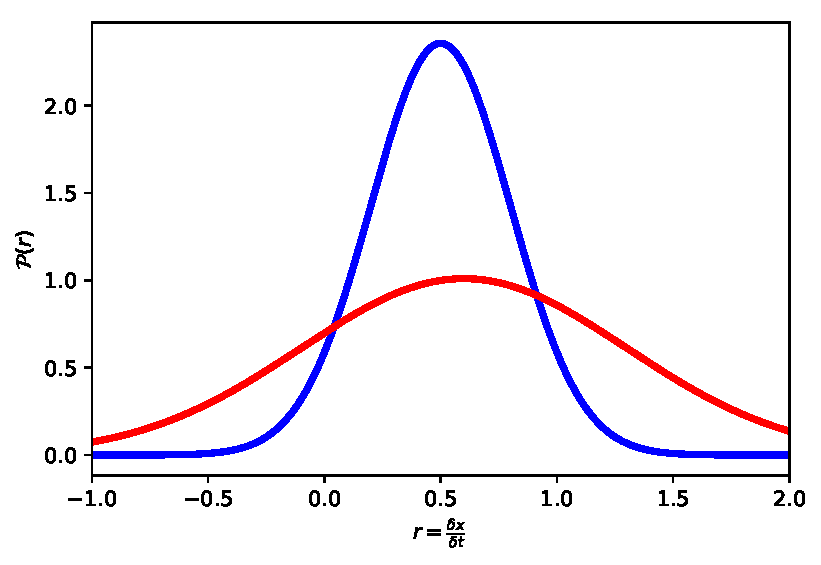
\includegraphics[width=\textwidth]{./chapter_rates/figs/two_dists.pdf}
%\caption{Two possible probability density functions for the per-round 
%multiplier, $\gr$, defined in \eref{R_def}. The distribution denoted by 
%the blue line has a higher mean and a higher variance than the one 
%in red. How are we to decide which represents the more favourable 
%gamble?\flabel{dec_dist}}
%\end{figure}



\section{Decisions in a deterministic world}
\seclabel{Decisions_in_a_deterministic}
\subsection{Different magnitudes}
I'm off to the bank to withdraw some money for you. I offer to give you either
\bi
\item[(1)] \$20 when I 
get back or 
\item[(2)] \$50 when I get back. You tell me what you prefer.
\ei
Let's see what our decision axiom says you'll do. Remember there's no uncertainty, I'm not lying to you, no one will rob me on my trip to the bank \etc

I haven't told you how long it will take me to get to the bank, so let's keep that general and call that time interval $\Dt$.
Because we know that $\Dt$ is the same under options (1) and (2) we don't actually need to know its value to compare the growth rates for the two options. 
We don't even have to know much about the functional form of the growth rate - we know that different situations require different forms of growth rates. The simplest examples are multiplicative and additive growth rates, and the general form of a growth rate is 
\be
\g=\frac{\D\gv(\x)}{\Dt},
\elabel{gen_rate}
\ee
where $\gv(\x)$ is a monotonically increasing function of wealth $\x$ that ensures temporal stability of $\g$. 
How does this work? Imagine $\x(\t)$ grows according to some dynamic. In order to say meaningfully how fast $\x$ is growing, this rate has to be stable in time. For example, if $\x(\t)$ grows exponentially, the additive rate of change $\frac{\D\x}{\Dt}$ will change throughout time. 

Therefore, we have to choose $\gv(\x)$ appropriately. In full generality, we demand that \eref{gen_rate} 
be a constant, namely the relevant growth rate. The functional form of the growth rate, \ie the function 
$\gv(\t)$, is given by the dynamic. To see this, we work backwards. Let's say \eref{gen_rate} is constant. 
Considering infinitesimal changes, we have
\be
\g=\frac{d\gv(\x)}{d\t}.
\elabel{gen_rate_inf}
\ee
We can separate variables and integrate this to find
\be
\gv(\x)=\g \t
\elabel{gen_rate_inf}
\ee
(where we've set the constant of integration to zero -- we're only ever interested in changes in $\gv$ so this constant will always cancel out).
This in turn tells us what the dynamic must be. The function $\gv(\x)$, we know evaluates to $\g\t$. Its inverse function evaluated at $\g\t$ therefore must be $\x$, the desired dynamic
\be
\x=\gv^{[-1]}(\g \t).
\elabel{gen_rate_inf}
\ee
It clearly works for multiplicative and additive growth. But let's take another example: what process has the growth rate $\frac{\D\x^{1/2}}{\Dt}$?
Well, with $\gv=\x^{1/2}$, we have $\gv^{[-1](\g \t)}=(\g\t)^2$, and thus the dynamic has to be $\x(\t)=(\g\t)^2$. Let's check and compute the appropriate growth rate: 
\bea
\g&=&\frac{\D\gv(\x)}{\Dt}\\
&=&\frac{\D[(\g\t)^2]^{1/2}}{\Dt}\\
&=&\g
\eea
as desired.

In the present case it turns out that any growth rate will give the same answer. Let's see.
Under option a) we have
\be
\g^{(1)} =\frac{\gv(\x+\$20)-\gv(\x)}{\Dt},
\ee
and under option b) we have
\be
\g^{(2)} =\frac{\gv(\x+\$50)-\gv(\x)}{\Dt}.
\ee
To find out which growth rate is larger, we subtract $\g^{(a)}$ from $\g^{(b)}$ 
\bea
\g^{(2)}-\g^{(1)} &=&\frac{\gv(\x+\$50)-\gv(\x)(-\gv(\x+\$20)-\gv(\x))}{\Dt}\\
 &=&\frac{\gv(\x+\$50)-\gv(\x+\$20)}{\Dt}.
\eea
Because $\gv(\x)$ is monotonically increasing, any growth rate will be greater under option (2), and 
our model humans will always go for option (2). That's good -- because I would have chosen option (2) if I were you, and 
our model reproduces this intuitive result.

More generally, our model says: of two certain payments of different sizes at the same time, choose the bigger one.

\subsection{Different magnitudes and times - discounting}
\seclabel{Different_magnitudes_and}
Let's make the decision a little harder: what if I offer you 
\bi
\item[(1)] \$10 in a month or 
\item[(2)] \$25 in two months?
\ei
Again, we will compute the two growth rates corresponding to options (1) and (2), and then choose the bigger one -- that's how we have been programmed to behave in the world that our axiom is creating. But unlike in the previous case, the functional form of the growth rate will now be important. 

Let's start with the exponential growth rate, with $\gv(\x)=\ln \x$ in \eref{gen_rate} -- this is the appropriate rate if wealth grows exponentially, like in a savings account.
We now have growth rates
\be
\gm^{(1)} =\frac{\ln(\x+\$10)-\ln(\x)}{1 \text{ month}},
\ee
and
\be
\gm^{(2)} =\frac{\ln(\x+\$25)-\ln(\x)}{2 \text{ months}}.
\ee
Curiously, which is greater depends on your initial wealth, in our model world. If your wealth is \$100, then $\gm^{(1)}\approx 114\%$ p.a., and 
$\gm^{(2)}\approx 134\%$ p.a., wherefore you will choose option (2).

But if your initial wealth is \$1, then $\gm^{(1)}\approx 2,877\%$ p.a. and $\gm^{(2)}\approx 1,955\%$ p.a., and you'll choose option (1).

We learn: in this slightly more complex though still fully deterministic case, which option is 
preferable does not only depend on the options available but also on the personal 
circumstances (initial wealth) of the decision maker.

\begin{figure}
\centering
\begin{picture}(200,80)(0,0)
 \put(-75,0){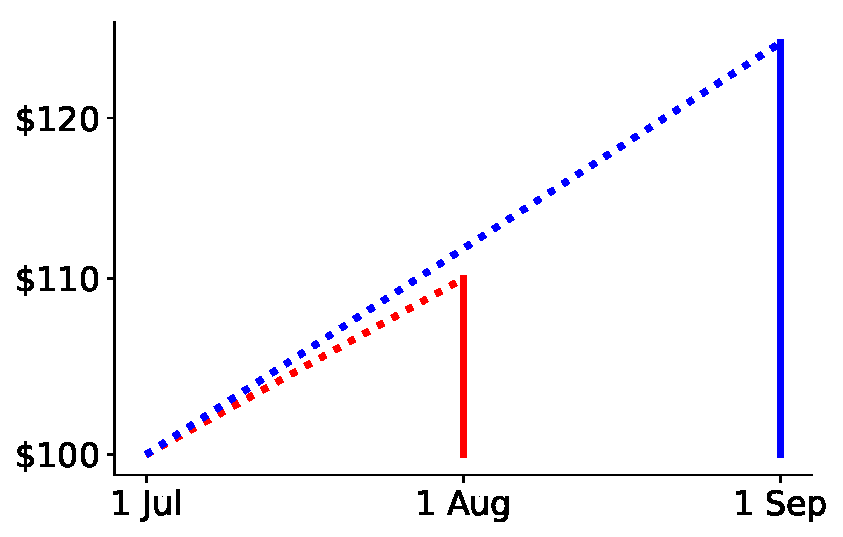
\includegraphics[width=.45\textwidth]{./chapter_rates/figs/exp_disc_2.pdf}}
 \put(120,0){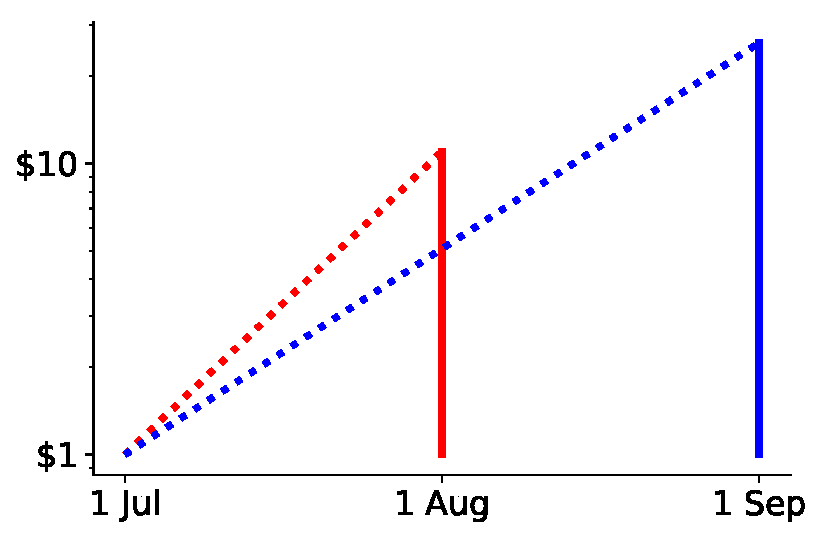
\includegraphics[width=.45\textwidth, angle=0]{./chapter_rates/figs/exp_disc_1.pdf}}
 \put(-35,80){A}
 \put(155,80){B}
\end{picture}
\caption{\small Slopes with logarithmic vertical scales. (A) If you have a lot of money (here \$100), exponential growth-rate optimization tells you to be patient and choose the later, larger, payment of \$25. (B) If you have little money (here \$1), the same criterion -- exponential growth-rate optimization -- tells you to get the cash as fast as possible, and choose the earlier, smaller, payment of \$10.}
\flabel{hyp_disc}
\end{figure}


Notice how the poorer decision maker seems to be more impatient, despite his use of the exact same decision axiom.
Using $\gv(\x)=\ln(\x)$ in \eref{} is related to what's called ``exponential discounting'' in the economics literature \cite{MavroyiannisETAL2019}.

What about the additive growth rate? That would be the relevant growth rate to compute if, for instance, these payments to us are promised as a salary. I already know what you'd pick: \$1 per month, or \$3 per two months? The reason I know what you'd choose is that it doesn't depend on your initial wealth. Let's see, that's just working with the identity function $\gv(\x)=\x$ in \eref{gen_rate}.
\be
\gad^{(1)} =\frac{\x+\$1-\x}{1 \text{ month}} \approx \$0.083 \text{ p.a.},
\ee
and
\be
\gad^{(2)} =\frac{\x+\$3-\x}{2 \text{ months}}\approx \$0.167 \text{ p.a.}.
\ee
Initial wealth cancels out: this is a unique feature of the additive growth rate. Only under additive dynamics does initial wealth not enter into the computation of the growth rate, and growth rates can be computed with knowledge of only the payouts and waiting times.

In the economics literature, decision-making based on additive growth rates is called ``hyperbolic discounting'' because this case is mathematically equivalent to discounting payments in the future with the hyperbolic function $\frac{1}{\Dt}$.

An interesting feature of optimizing additive growth rates is what's called ``preference reversal:'' let's keep our example as it is, except we now let time march forward, holding fixed the moments in time when the payments are to be made. Under these conditions, there comes a time, precisely after half a month, when option (2) is no longer preferred, see \fref{hyp_disc}.

\begin{figure}
\centering
\begin{picture}(200,80)(0,0)
 \put(-80,0){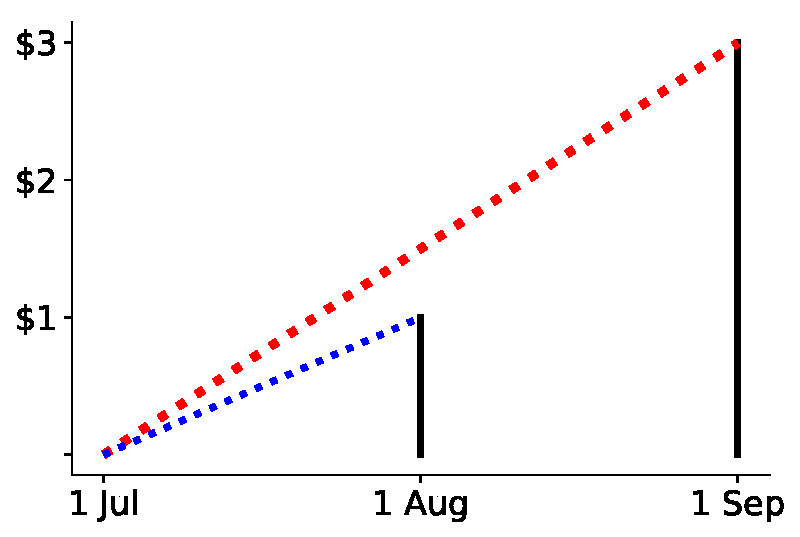
\includegraphics[width=.33\textwidth]{./chapter_rates/figs/disc_1.pdf}}
 \put(40,0){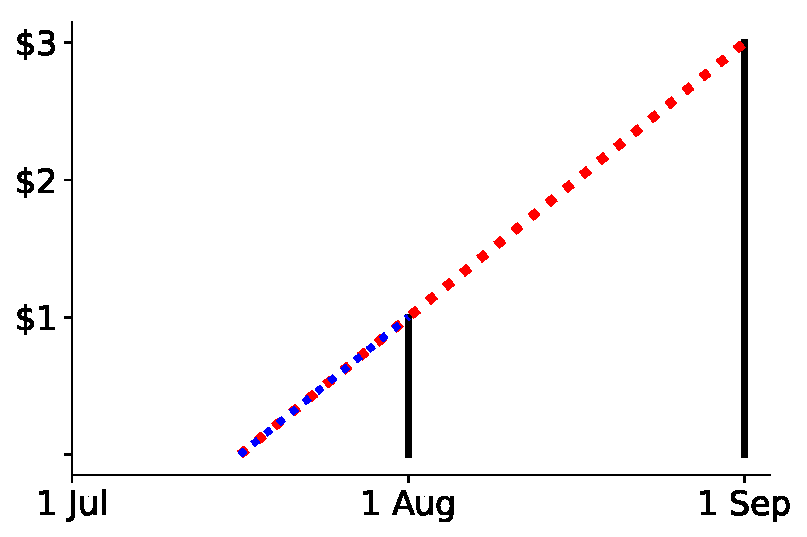
\includegraphics[width=.33\textwidth, angle=0]{./chapter_rates/figs/disc_2.pdf}}
 \put(160,0){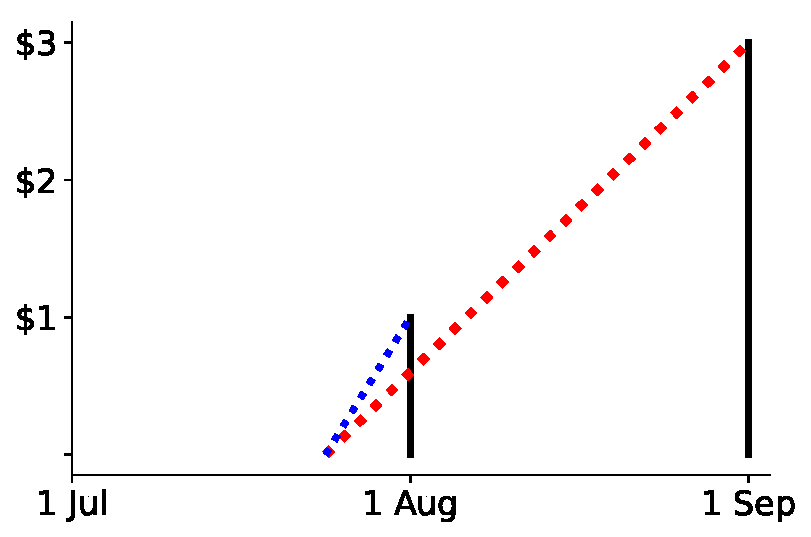
\includegraphics[width=.33\textwidth, angle=0]{./chapter_rates/figs/disc_3.pdf}}
\put(-60,60){A}
\put(60,60){B}
\put(180,60){C}
\end{picture}
\caption{\small  Slopes with linear vertical scales. (A) At the beginning option (2) yields the highest additive growth rate; (B) after half a month, the options are equally good; (C) after 3/4 of a month, preference reversal has taken place, and option (1) now yields the highest growth rate. As the first payment approaches, the associated growth rate diverges.}
\flabel{hyp_disc}
\end{figure}

Perhaps the most significant message is the richness of this problem. We're applying nothing but our simple axiom, but it forces us to choose how we think about the dynamics of our wealth, and in reality that may depend strongly on many difficult to specify circumstances. In real life payments are not just offered at some point in time, but usually in return for something -- an asset or work. Depending on the specific exchange, an additive, multiplicative, or more general model will be appropriate.

Importantly, we need not resort to psychology to generate a host of behaviours, such as impatience of poorer individuals or preference reversal as time ticks on.

\section{Decisions in an uncertain world}
\seclabel{Decisions_in_an}
In the previous section we saw some interesting types of behaviour that occur in a model world generated by our decision axiom. We were able to relate these to phenomena that already have names in the more complex model worlds of classical economics, for instance ``discounting'' and ``preference reversal.''

In the present section we will make our model world more realistic by introducing randomness. We will do this in a way that's natural from the perspective of growth rate optimization, and it will lead us to re-discover another concept of the classical theory, namely the gamble.

We clearly have to do something about our axiom: with randomness the growth rates that are the basis of decisions in our model will also be random. We get around that problem by interpreting ``growth rate'' in the axiom as ``time-average growth rate'' when there's randomness involved. The functional form of the rate that guarantees stability in time of rates  in the deterministic case will now guarantee ergodicity of rates, see below. This will allow us to use expectation values of rates when they are easier to compute.

\begin{keypts}{Decision axiom {\it with randomness}}

People optimize the {\it time-average} growth rate of their wealth.

\end{keypts}

Our model rationale for deciding between two gambles is simple: 
given a model for the mode of repetition, 
choose the gamble with the largest time-average growth rate. 
In other words, choose the gamble which, 
if repeated indefinitely, causes your wealth to grow fastest.

We are not saying that real repetitions are necessary. We 
merely create model humans who base decisions on what would 
happen to their wealth if they were repeated (infinitely many times). It is a 
conceptual device -- in effect a thought experiment -- to elicit the 
underlying tendency of each gamble. A particular choice that can be 
represented by gambles 
may be offered only once and, indeed, in the real world this will 
often be the case. However, in the real world it is also the case 
that a decision is likely to be followed by many others, a scenario 
to which indefinite repetition is a plausible approximation.

In our thought experiment this decision rule outperforms any other 
decision rule almost surely: so, at least in that imagined world, the 
rationale has a physical basis. If our thought experiment is a good 
approximation to real-world decision scenarios, then our rationale 
should be a good model of real-world decisions. Certainly it is 
parsimonious, based on a single, 
robust quantity and requiring only the gamble and its mode of repetition 
to be specified. Unlike some treatments of human decision-making, it 
contains no arbitrary or hard-to-measure psychological factors.

Having said all this, while we think that the decision axiom 
is reasonable, we stress that at this point it is an \textit{axiom}, \ie something we assert without empirical justification and which is not deduced from more primitive considerations. It 
defines a model world where certain types of behaviour will be observed. 
We will show in \secref{Copenhagen} and in \cref{Markets} why we feel reminded 
of reality by this model world, though you may disagree 
and you may prefer a different model that creates a different model world
that reminds you more of reality.
Other decision axioms are 
possible and, indeed, have been proposed. For instance, 
classical decision theory is defined by the axiom that decision
makers maximize expected utility -- though \secref{Copenhagen} 
shows that this model has flaws that may not be acceptable. 

%Copenhagen experiment? Little excursion?

Our decision rationale can be expressed as a set of instructions.
We denote quantities relating to the $\m^\text{th}$ available gamble with the 
superscript $(\m)$. Each gamble is specified by its random payout, $\Q^{(\m)}$, and 
per-round period, $\dt^{(\m)}$. 

\begin{keypts}{Growth-optimal decision algorithm}
\begin{enumerate}
\item Specify $\Q^{(\m)}$ and $\dt^{(\m)}$ for the gambles offered;
\item Specify the wealth dynamic, \ie the relationship between $\d\x(\t)$, 
$\x(\t)$, and $\q$;
\item Find the ergodicity transformation, $\gv(\x)$, of the wealth whose increments are 
instances of a (time-independent) random variable under this dynamic;
\item Determine the time-average growth rates, $\gt^{(\m)}$, either by taking 
the long-time limit of the growth rates, $\g^{(\m)}(\t,\Dt)$, or by invoking the 
ergodic property and taking their ensemble averages;
\item Choose the gamble, $\m$, with the largest time-average growth rate.
\end{enumerate}
\end{keypts}

In examples, we will focus on choices between two 
gambles, \ie $\m\in\{1,2\}$. Decisions between three or more gambles 
are straightforward extensions.
Often one of the gambles presented is the null gamble, which trivially 
has a growth rate of zero. In this case, the question is 
whether the other gamble is preferable to doing nothing, 
\ie bet or no bet?

We will illustrate the decision algorithm by applying it to the coin toss 
game of \cref{Coins}. $\x(\tn)>\$ 0$ is the starting 
wealth and $\dt$ is the time between rounds for each of the 
gambles offered. We recall that the coin toss gamble is specified by the random payout:
\bea
\q^{(1)}_1 = -0.4\x(\tn), &\quad& \p^{(1)}_1 = 1/2; \\
\q^{(1)}_2 = 0.5\x(\tn), &\quad& \p^{(1)}_2 = 1/2.
\eea
Note that, in our setup, the payouts $\Q^{(\m)}_\gi$ are always fixed 
monetary amounts. Here they are expressed as fractions of $\x(\tn)$, 
which is itself a fixed monetary wealth.\footnote{Even though this 
formulation might appear to encode a multiplicative dynamic (largely 
because it comes from an imagined multiplicative game), we have 
arranged things so that formally it does not. Indeed, it encodes no 
dynamic at all: that is specified separately.} We shall ask our individual 
to choose between the coin toss and the null gamble,
\be
\q^{(2)}_1 = \$0, \quad \p^{(2)}_1 = 1.
\ee
Both the additive and multiplicative versions of the repeated gamble are analysed.

\begin{example}{Additive coin toss game}
If the repetition is additive, wealth will evolve over $T$ rounds according to:
\bea
\x^{(1)}(t_0+\T\dt) &=& \x(\tn) + \sum_{\gtau=1}^\T \q^{(1)}(\gtau); \\
\x^{(2)}(t_0+\T\dt) &=& \x(\tn).
\eea
Here we have assumed that wealth is free to go negative, \ie that 
there is no bankrupt state from which the individual can't 
recover.\footnotemark\ The ergodicity transformation is the identity, 
$\gv(\x)=\x$, so the growth rates are simply the rates of change of 
wealth itself. We can express these over the $\T$ rounds as:
\bea
\gad^{(1)}(\t) = \frac{\x^{(1)}(\t+\T\dt) - \x(\tn)}{\T\dt} &=& \frac{1}{\T}\sum_{\gtau=1}^\T \frac{\q^{(1)}(\gtau)}{\dt}; \elabel{g1_add}\\
\gad^{(2)}(\t) = \frac{\x^{(2)}(\t+\T\dt) - \x(\tn)}{\T\dt} &=& \$ 0
\eea
per unit time. The long-time limit of the growth rate for the null gamble 
is trivially $\gad^{(2)}=\$0$ per unit time. For the coin toss, we calculate it as
\bea
\overline{\gad}^{(1)} &=& \lim_{\T\to\infty}\left\{\frac{1}{\T}\sum_{\gtau=1}^\T \frac{\q^{(1)}(\gtau)}{\dt}\right\}\\
&=& \ave{\frac{\q^{(1)}}{\dt}}\\
&=& \frac{\p^{(1)}_1 \q^{(1)}_1 + \p^{(1)}_2 \q^{(1)}_2}{\dt}\\
&=& \frac{0.05\x(\tn)}{\dt},
\eea
which is positive (assuming $\x(\tn)>\$0$). Therefore, $\overline{\gad}^{(1)}>\overline{\gad}^{(2)}$ 
and our individual should accept the coin toss gamble under additive dynamics.
\end{example}
\footnotetext{We could model this realistic feature by an absorbing boundary on $\x(\t)$, if we were so minded.}

We see from this example that the decision rule under additive repetition is to 
maximise $\ave{\q/\dt}$.\footnote{Too frequently in presentations of decision 
theory, it is assumed implicitly that $\dt$ is the same for all available gambles 
and the decision algorithm is presented as the maximisation of the expected 
payout, $\ave{\q}$. While this is equivalent if all the $\dt^{(\m)}$ are identical, it 
is not if they aren't. Moreover, the assumption is usually left unstated. This is 
unhelpful in that it masks the important role of time in the analysis and, in 
particular, the fact that our individual is maximising a \textit{rate}.} This is the 
rate of change of the expected wealth, which, as we know from \eref{g_bar_a}, 
happens to coincide under this dynamic with the time-average growth rate. We 
will see later that humans tend not to act to maximise $\ave{\q/\dt}$ in reality. 
This may not be a great shock: additive repetition without bankruptcy isn't 
going to win many prizes for the most realistic model of wealth evolution.

Let's try multiplicative repetition instead.

\begin{example}{Multiplicative coin toss game}
The payout, $\Q^{(1)}$, is re-expressed as a per-round multiplier,
\be
\gr^{(1)} = \frac{\x(\tn)+\q^{(1)}}{\x(\tn)},
\ee
which takes the values:
\bea
\gr^{(1)}_1 = \frac{\x(\tn)+\q^{(1)}_1}{\x(\tn)} = 0.6, &\quad& \p^{(1)}_1 = 1/2; \\
\gr^{(1)}_2 = \frac{\x(\tn)+\q^{(1)}_2}{\x(\tn)} = 1.5, &\quad& \p^{(1)}_2 = 1/2.
\eea
Under multiplicative dynamics, the wealth evolves according to:
\bea
\x^{(1)}(\tn+\T\dt) &=& \x(\tn) \prod_{\gtau=1}^\T \gr^{(1)}(\gtau); \elabel{W1T_mult}\\
\x^{(2)}(\tn+\T\dt) &=& \x(\tn).\elabel{W2T_mult}
\eea
The ergodicity transformation is the logarithm, $\gv(\x)=\ln \x$. We have 
already discussed why, but one way of seeing this is to take logarithms of 
\eref{W1T_mult}. This converts the product into a sum of independent instances of a random variable:
\bea
\ln \x^{(1)}(\tn+\T\dt) &=& \ln \x(\tn) + \sum_{\gtau=1}^\T \ln \gr^{(1)}(\gtau); \elabel{lnW1T_mult}\\
\ln \x^{(2)}(\tn+\T\dt) &=& \ln \x(\tn).\elabel{lnW2T_mult}
\eea
Therefore, $\ln \x$ is the desired quantity whose increments 
inherit their ergodicity from $\q$. The growth rates, expressed over $\T$ rounds, are:
\bea
\gm^{(1)}(\t) = \frac{\ln \x^{(1)}(\t+\T\dt) - \ln \x(\tn)}{\T\dt} &=& \frac{1}{\T}\sum_{\gtau=1}^\T \frac{\ln \gr^{(1)}(\gtau)}{\dt};\\
\gm^{(2)}(\t) = \frac{\ln \x^{(2)}(\t+T\dt) - \ln \x(\tn)}{\T\dt} &=& 0
\eea
per unit time. As in the additive case, we take the $\T\to\infty$ limits. For the null 
gamble this is trivial: $\gt_\text{m}^{(2)}=0$ per unit time. For the coin toss gamble, we get
\bea
\gt_\text{m}^{(1)} = \ave{\frac{\ln \gr^{(1)}}{\dt}} = \frac{\ln\left(\sqrt{0.9}\right)}{\dt},
\eea
which is negative. Thus, $\overline{\gm}^{(1)}<\overline{\gm}^{(2)}$ under multiplicative 
dynamics and our individual should decline the coin toss. That this is the opposite 
of his decision under additive repetition highlights the importance of specifying a 
dynamic that corresponds well to what is happening in reality.

Another way of presenting the repeated coin toss is to express the wealth 
after $\T$ rounds as
\be
\x^{(1)}(\tn+\T\dt) = \x(\tn)\left(\gr_\T^{(1)}\right)^\T,
\ee
where
\be
\gr_\T^{(1)} = (0.6)^{(\T-\gk)/\T}(1.5)^{\gk/\T}
\ee
is the equivalent per-round multiplier after $\T$ rounds and 
$0\leq \gk\leq \T$ is the number of winning rounds. $\gr_\T$ 
is a random variable but it converges almost surely to a scalar in the long time limit,
\be
\gr_\infty^{(1)} \equiv \lim_{\T\to\infty}\{\gr_\T^{(1)}\} = (0.6)^{1/2}(1.5)^{1/2} = \sqrt{0.9},
\ee
since $\gk/\T\to1/2$ as $\T\to\infty$ (the coin is fair). $\gr_\infty^{(1)}<1$ so the 
individual's wealth is sure to decay over time and he should decline the gamble. 
The two approaches are, of course, linked, in that
\be
\gt_\text{m}^{(1)} = \frac{\ln \gr_\infty^{(1)}}{\dt}.
\ee
\end{example}

Here we see that our decision rule boils down to maximising
\be
\ave{\frac{\ln \gr}{\dt}} = \ave{\frac{\ln(\x(\tn)+\q)-\ln \x(\tn)}{\dt}}.
\ee
This coincides with the time-average growth rate in \eref{g_bar_m}.

===============================================

\section{Gamble: random number and duration}
\seclabel{Gamble:}
One fundamental building block of mathematical decision theory is the gamble.
This is a mathematical object that resembles a number of situations in real life, 
namely situations where we face a decision whose consequences will be purely
financial and are somewhat uncertain when we make the decision. A real-world example would be buying a lottery ticket. We define the gamble mathematically as follows.

\begin{defn}{Gamble}
A gamble is a pair of a random variable, $\Q$, and a duration,  $\dt$. 
\vspace{.2cm}

$\Q$ is called the payout and takes one of $\K$ (mutually exclusive) possible monetary 
values, 
$\{\q_1,\ldots,\q_{\K}\}$, associated with probabilities, $\{\p_1,\ldots,\p_{\K}\}$, where 
$\sum_{\gj=1}^\K \p_\gj = 1$. 
Payouts can be positive, associated with a monetary gain, or negative, 
associated with a loss. We order them such that $\q_1<\ldots<\q_\K$.
\end{defn}

Everything we need to know about the gamble is contained in the 
payouts, probabilities, and duration. In economics, the duration of a gamble is rarely discussed but it's clearly crucial information, as a trivial example shows. Let's say you get to choose between two gambles. One pays $\$1$ with probability $1$ and takes one second to complete; the other also pays $\$1$ also with probability $1$ but takes one year to complete. Clearly the former is more attractive.

We relate the abstract gamble to reality through a few situations that may be modelled as gambles:

\begin{example}{Betting on a fair coin}
Imagine betting $\$ 10$ on the toss of a fair coin. We would model this 
with the following payouts and probabilities:
\bea
\q_1 = -\$ 10, &\quad& \p_1 = 1/2;\\
\q_2 = +\$ 10, &\quad& \p_2 = 1/2.
\eea
The duration may be the time until you receive the payout, or if you participate in coin tosses once a week we may want to make it $\dt=1$ week.
\end{example}

\begin{example}{Playing the lottery}
We can also imagine a gamble akin to a lottery, where we pay an amount, 
$\F$, for a ticket which will win the jackpot, $\J$, with probability, $\p$. The corresponding 
payouts and probabilities are:
\bea
\q_1 = -\F,  &\quad& \p_1 = 1-\p;\\
\q_2 = \J-\F, &\quad& \p_2 = \p.
\eea
Note that we deduct the ticket price, $\F$, in the payout $\q_2$.
The duration may be $\dt=1$ week.
\end{example}

\begin{example}{Betting at fixed odds}
A bet placed at fixed odds, for example on a horse race can also be modelled as a gamble. 
Suppose we bet on the horse \textit{Ito} to win the 2015 Prix de l'Arc de Triomphe 
in Paris at odds of 50/1 (the best available odds on 20th September 2015). 
\textit{Ito} will win the race with unknown probability, $\p$. If we bet $\F$, 
then this is modelled by payouts and probabilities:
\bea
\q_1 = -\F,  &\quad& \p_1 = 1-\p;\\
\q_2 = 50\F, &\quad& \p_2 = \p.
\eea
The duration may be something like $\dt=30$ minutes.
\end{example}

\begin{example}{The null gamble}
It is useful to introduce the null gamble, in which a payout of zero is received 
with certainty: $\q_1=\$0$, $\p_1=1$. This represents the `no bet' or `do nothing' option.

As in the examples above, the duration, $\dt$, has to be chosen appropriately. 
The meaning of the duration will become clearer later on -- often it is the time 
between two successive rounds of a gamble.
\end{example}

The gamble is a simple but versatile mathematical model of an uncertain future. 
It can be used to model not only traditional wagers, such as sports bets and 
lotteries, but also a wide range of economic activities, such as stock market 
investments, insurance contracts, derivatives, and so on. The gamble we have 
presented is discrete, in that the payout, $\Q$, is a random variable with a 
countable (and, we usually assume, small) number of possible values. 
The extension to continuous random variables is natural and used frequently 
to model real-world scenarios where the number of possible outcomes, \eg the change 
in a stock price over one day, is large.

Suppose now that you have to choose between two options that you've modelled 
as two gambles (possibly including the null gamble). Which should you choose, 
and why? This is the gamble problem, the central question of decision theory, and 
the basis for much of mainstream economics.

\begin{defn}{The gamble problem}
The gamble problem is the problem to choose between two gambles.
\end{defn}

We stress here that the gamble alone is not enough information to answer this question. 
The value of a gamble -- clearly -- depends on more facts than probabilities, payouts, and duration. Crucially, it depends 
\begin{enumerate}
\item
on how the gamble affects our future. For instance: if we go bankrupt as a result, can we recover from that?
\item
on our circumstances. When you're very rich you can afford to take risks that you can't afford when you're poor. 
\item
on our personality. Some like the thrill of gambling, others find it unpleasant.
\end{enumerate}
Mainstream economics focuses on point 3, whereas we focus on points 1 and 2.

Although the gamble problem is underspecified by a gamble alone, the gamble is a 
useful conceptual unit because it specifies that part of the model of evolving wealth 
that is independent of individual circumstances. It thus splits an easily observable part
of the problem from information that's much harder to obtain. We can all buy the same lottery 
ticket with publicly specified prizes, probabilities, duration -- for some of us that will be attractive, for others it won't, for a variety of reasons.

%%%%%%%%%%%%%%%%%%%%%%%%%%%%%%%%%%%%%%%%%%%%%%%
\section{Repeated gamble: from random number to stochastic process}
\seclabel{Repeated_gamble}
To solve the gamble problem we must propose a criterion to choose between two
gambles. Different criteria will result in different decisions -- by writing down a criterion
we build a model world of model humans who behave in ways that may seem sensible
to us or crazy -- if the behaviour seems crazy we have probably not chosen a good
criterion and we should look back, think about what may be wrong with the criterion, 
and try a better one.

The wealth process $\x(\t)$ is related to the gambles our model humans 
choose to play. Precisely {\it how} it is related remains to be specified.

Considering a single round of a gamble in isolation -- the so-called `one-shot' setup 
-- is relatively uninstructive in this regard, though that hasn't diminished its prominence in wider literature. 
All we know is 
that one of the possible payouts will be received, leading to the random value 
$\x(\t+\dt)=\x(\t)+\q$. 
We don't yet know how accepting this gamble will affect how our wealth, $\x(\t)$, grows or decays over time, since one time step isn't enough for this to become apparent. 
The one-shot game takes one random value, $\q$, and turns it trivially into 
another, $\x(\t)+\q$. Time has no significance in a 
one-shot game. An amount $\dt$ elapses, but this could be a single 
heartbeat or the lifetime of the universe, for all the difference it makes to the analysis.

To establish how your wealth evolves, we must imagine that the world does 
not come to a grinding halt after the gamble. Instead we imagine that the gamble
is repeated over many rounds.\footnote{In fact, to make the 
problem tractable mathematically, it will be necessary to imagine the gamble 
is repeated indefinitely.} This does not mean that we actually
believe that a real-world situation will repeat itself over and over again, \eg we don't
believe that we will bet on the horse \textit{Ito} at odds 50/1 many times in a row. Instead, 
imagining repetition is a methodological device that allows us to extract tendencies
where they would otherwise be invisible. It is the model analogue of 
the idea that individuals live in time and that their decisions have consequences 
which unfold over time.

Crucially, {\it the mode of repetition is not specified in the gamble itself.} It is a 
second component of the model, which must be specified separately. Initially we shall 
focus on two modes: \textit{additive} and \textit{multiplicative} repetition. Other dynamics will be considered later on, in \secref{general_dynamics}.

\begin{defn}{Additive repetition}
If a gamble is repeated additively then  
a newly generated realization of the random payout, $\q$, is added to $\x(\t)$ 
at each round. We define the change in wealth occurring 
over a single round as
\be
\d \x(\t) \equiv \x(\t+\dt)-\x(\t).
\elabel{DW_def}
\ee
In the additive case, we have
\be
\d\x(\t) = \q.
\elabel{DW_add}
\ee
In other words, under additive repetition, $\d \x$ is a stationary 
random variable.
%\footnote{This seemingly mundane corollary stems 
%from our definitions of $\gD$ as a monetary payout and $\d\x$ as an 
%additive change in wealth, expressed in monetary units. It would not 
%hold if, for example, we had defined $\d\x$ to be some other type of 
%change, such as a relative change.}
Starting at time, $\tn$, wealth 
after $\T$ rounds is
\be
\x(\tn+\T\dt) = \x(\tn) + \sum_{\gtau=1}^\T \q(\gtau),
\elabel{Wt_add}
\ee
where $\q(\gtau)$ is the realisation of the random variable in round $\gtau$. 
This is an evolution equation for wealth following a noisy additive dynamic. 
Note that $\x(\tn+\T\dt)$ is itself a random variable.
\end{defn}


\begin{example}{Additive repetition}
We return to our first example of a gamble: a $\$ 10$ bet on 
a coin toss. Under additive repetition, successive bets will always 
be $\$ 10$, regardless of how rich or poor you 
become. Suppose your starting wealth is $\x(\tn)=\$ 100$. 
Then, following \eref{Wt_add}, your wealth after $\T$ rounds will be
\bea
\x(\tn+\T\dt) &=& \$ 100 + \$ 10 \gk - \$ 10 (\T-\gk)\\
&=& \$ [100 +  10(2\gk-\T)],
\eea
where $0\leq \gk\leq \T$ is the number of tosses you've won. Note that
we have assumed your wealth is allowed to go negative. If not, then the 
process would stop when $\x<\$ 10$, since you would be unable 
to place the next $\$ 10$ bet.
\end{example}

An alternative is multiplicative repetition. In the example above, let 
us imagine that the first $\$ 10$ bet were viewed not as a bet 
of fixed monetary size, but as a fixed fraction of the 
starting wealth ($\$ 100$). Under multiplicative repetition, each 
successive bet is for the same fraction of wealth which, 
in general, will be a different monetary amount.

The formalism is as follows. The payout, $\q_{\gj}$, in the first round is 
expressed instead as a random wealth multiplier,
\be
\gr_{\gj} \equiv \frac{\x(\tn)+\q_{\gj}}{\x(\tn)}.
\elabel{R_def}
\ee
The multiplier is another random variable -- it also (trivially) defines a stochastic process that is a new instance of the random variable at each point in time, $\gr(\t)$. The gamble is repeated by applying another instance of the same multiplier at all subsequent rounds:
\be
\x(\t+\dt) = \gr(\t)\x(\t).
\ee
From \eref{R_def} we see that $\gr(\t)$ is a sequence of instances 
of a random variable with time-independent distribution, 
since it depends only on $\Q$, which is time-independent, and the starting 
wealth, $\x(\tn)$, which is fixed. However, distributions of successive changes in wealth,
\be
\d \x(\t) = (\gr-1)\x(\t),
\elabel{DW_mult_short}
\ee
are not time-independent, as they depend on $\t$ through $\x(\t)$. The wealth 
after $\T$ rounds of the gamble is
\be
\x(\tn+\T\dt) = \x(\tn)\prod_{\gtau=1}^\T \gr(\gtau),
\ee
where $\gr(\gtau)$ is the realisation of the random multiplier in round $\gtau$.

\begin{example}{Multiplicative repetition}
The $\$10$ bet on a coin toss is now re-expressed as a bet of a fixed 
fraction of wealth at the start of each round. Following 
\eref{R_def}, the random multiplier, $\gr$, has two possible outcomes:
\bea
\gr_1 = \frac{\$100 - \$10}{\$100} = 0.9, &\quad& \p_1 = 1/2;\\
\gr_2 = \frac{\$100 + \$10}{\$100} = 1.1, &\quad& \p_2 = 1/2.
\eea
The wealth after $\T$ rounds is, therefore,
\be
\x(\tn+\T\dt) = \$100\,\,(1.1)^\gk\,(0.9)^{\T-\gk},
\ee
where $0\leq \gk \leq \T$ is the number of winning tosses. In this example there is 
no need to invoke a `no bankruptcy' condition, since our individual can lose no 
more than 10\% of his wealth in each round.
\end{example}

The difference between the two modes of repetition might easily be mistaken 
for a matter of taste. When the $\$ 10$ bet was first offered, what 
difference does it make whether our individual imagined this to be a bet of a 
fixed size or of a fixed fraction of his wealth? However, the consequences of 
this choice between imagined situations are enormous, as we shall see 
experimentally in \secref{Copenhagen}. In \cref{Coins} we saw that additive and multiplicative dynamics differ as starkly as the 
linear and exponential functions, and there is evidence that people adjust their behaviour
to the type of repetition they face. 
%CPH
It matters, therefore, that we consider 
carefully the economic situation we wish to model in order to choose the 
most realistic mode of repetition. For example, fluctuations in the price of a 
stock tend to be proportional to the price, \cf \eref{DW_mult_short}, so 
multiplicativity is the appropriate paradigm for large wealth fully invested in stocks.

Now that we've established how the gamble is related to $\x(\t)$ we can 
begin to think about decision criteria. Not surprisingly, appropriate
growth rates are useful decision criteria -- ``pick the gamble that will make
your wealth grow fastest'' is generally good advice. To be able to 
follow this advice we will think again about growth rates.

%%%%%%%%%%%%%%%%%%%%%%%%%%%%%%%%%%%%%%%%%%%%%%%

%%%%%%%%%%%%%%%%%%%%%%%%%%%%%%%%%%%%%%%%%%%%%%%
\section{The expected-wealth and expected-utility paradigms}
Our decision rule under additive repetition of the gamble is to maximise
\be
\ave{\frac{\d\x}{\dt}} = \ave{\frac{\q}{\dt}},
\elabel{ex_crit}
\ee
\ie the rate of change of the expectation value of wealth. This was, in fact, the first 
decision rule to be suggested when gamble problems were considered in the early 
days of probability theory in the $17^\text{th}$ century. We will call this the 
`expected-wealth paradigm'. It was not derived as we have derived it, from a 
criterion to maximise growth over repetition. Instead, it was essentially proposed 
as the decision axiom itself, with no reference to dynamics. It is easy to see why: 
it is a simple rule containing a familiar type of average, which incorporates all the 
possible outcomes of the game. Indeed, it would be logically sound if we could play 
the game many times in parallel, thereby accessing all the possible outcomes.

In the language of economics, the expected-wealth paradigm treats humans as 
`risk neutral', \ie they have no preference between gambles whose expected 
changes in wealth are identical (over a given time interval). This treatment has 
been known to be a flawed model of human decision-making since at least 
1713~\cite[p.~402]{Montmort1713}, in that it does not accord well with observed behaviour.

The conventionally offered reason for this predictive failure is that the value to an 
individual of a possible change in wealth depends on how much wealth he already 
has and his psychological attitude to taking risks. In other words, people do not 
treat equal amounts of extra money equally. This makes intuitive sense: an extra 
$\$10$ is much less significant to a rich man than to a pauper for whom it 
represents a full belly; an inveterate gambler has a different attitude to risking 
$\$100$ on the spin of a roulette wheel than a prudent saver, their wealths 
being equal.

In 1738 Daniel Bernoulli~\cite{Bernoulli1738}, after correspondence with Cramer, devised the `expected-utility paradigm' to model these considerations. He observed that money may not translate linearly into usefulness and assigned to an individual an idiosyncratic utility function, $\gu(\x)$, that maps his wealth, $\x$, 
into usefulness, $\gu$. He claimed that this was the true quantity whose rate of change of expected value,
\be
\ave{\gr_\gu} \equiv \ave{\frac{\d\gu(\x)}{\dt}},
\elabel{euh}
\ee
is maximised in a choice between gambles.

This is the axiom of utility theory. It leads to an alternative decision algorithm, which we summarise here:
\begin{keypts}{Expected-utility decision algorithm}
\begin{enumerate}
\item Specify $\Q^{(\m)}$ and $\dt^{(\m)}$ for the gambles offered;
\item Specify the individual's idiosyncratic utility function, $\gu(\x)$, which maps his wealth to his utility;
\item Determine the rate of change of his expected utility over a single round of the gamble (no dynamic is specified so it's unclear how a gamble would be repeated),
\be
\ave{\gr_\gu}^{(\m)}=\ave{\frac{\gu\left(\x+\q^{(\m)}\right)-\gu(\x)}{\dt^{(\m)}}};
\ee
\item Choose the gamble, $\m$, with the largest $\ave{\gr_\gu}^{(\m)}$.
\end{enumerate}
\end{keypts}

Despite their conceptually different foundations, we note the similarities between the 
maximands\footnote{The quantities to be maximised.} of our growth-optimal decision 
theory, \eref{g_bar_gen}, and the expected-utility paradigm, \eref{euh}. Our decision theory
contains a mapping which transforms wealth into a variable, $\gv$, whose increments are 
instances of a time-independent random variable. This mapping depends on the wealth dynamic which 
describes how the gamble is repeated. The expected-utility paradigm contains a function which transforms 
wealth into usefulness. This is determined by the idiosyncratic risk preferences of 
the individual. If we identify the ergodicity transformation of the former with the 
utility transformation of the latter, then the expressions are the same.

But we caution against the conceptual world of expected utility theory. It uses expectation
values, where they are inappropriate (because decisions of an individual are considered, 
not of many parallel systems), and it corrects for this error by introducing a non-linear 
mapping of wealth (the utility function) whose specific form cannot be pinned down 
convincingly. Finally, because of this conceptual weakness, utility theory is poorly defined. 
The very first paper on the topic contains two contradictory definitions of expected utility 
theory \cite{Bernoulli1738}, and over the centuries several others have been added.

Nonetheless, with a few assumptions, expected utility theory as we've
presented it above is consistent with growth rate optimisation, provided a suitable pair of dynamic and utility function is used. 
For multiplicative dynamics, the necessary utility function is the logarithm. That this is the most 
widely used utility function in both theory and practice is a psychological fluke in the classic mindset; from our perspective it indicates that 
our brains have evolved to produce growth-optimal decisions in a world governed 
by multiplicative dynamics, \ie where entities produce more of 
themselves. Incidentally, a common definition of life is ``that which produces more of itself,'' or as Harold Morowitz put it \cite[p.~5]{Morowitz1992} ``Living systems self-replicate, that is, they give rise to organisms like themselves.'' From our perspective, the prevalence of logarithmic utility reflects our evolution in an environment of living things.

Thus we can offer a different reason for the predictive failure of the expected-wealth 
paradigm. In our framework this corresponds to good decisions under additive 
repetition, which we claim is generally a poor model of how wealth evolves.\footnote{It 
would correspond, for example, to the interest payments in your bank account being 
independent of your balance!} It fails, therefore, because it corresponds to an unrealistic dynamic. 

It's worth being explicit about how our theory differs from expected utility theory. 
In our model what's stable about human behavior is this: humans optimize wealth over time. Utility theory says humans optimize utility across the ensemble. Given a dynamic, our paradigm predicts human behavior that can be mapped to a predicted utility function. Utility theory believes that behavior, specifically risk preferences, is an idiosyncratic thing: it does not depend on the dynamics but on the individual. This difference (behavior is determined by dynamics vs. behavior is determined by indiosyncrasy) means that in principle we can find out which theory is right. We can change dynamic and see if people change behavior. That would invalidate expected utility theory. We can also take several people and expose them to the same dynamic -- the extent to which they display utility functions that are incompatible with the dynamic would invalidate our theory, insofar as it is interpreted to predict human behavior. Our theory provides the optimal behavioral protocol, in terms of long-term wealth growth, but of course real humans will only optimize long-term wealth growth to a certain degree. Nevertheless, we are happy to report that a Danish group of experimentalists has recently carried out experiments where subjects were exposed to different wealth dynamics, to see whether the utility functions implied by their behavior changed as predicted by our theory. At the time of writing, we're still waiting for the results.

\section{General dynamics}
\seclabel{general_dynamics}
Before we come to example applications of decision theory, it is time to discuss 
dynamics that are neither additive nor multiplicative and their relation to general
utility functions. 

\subsection{Why discuss general dynamics?}
What are we trying to achieve with this? First of all, where the time perspective has come
up in history, \eg \cite{Whitworth1870,Kelly1956}, it was always in the context of multiplicative 
dynamics, which, as we saw in the previous section, corresponds to logarithmic utility. One 
persistent criticism from people trained to think in terms of utility has been: what if my utility 
function is not logarithmic? In other words, the time perspective has seemed overly restrictive 
to many people.

As a matter of epistemology, we want to be somewhat restrictive. Imagine the opposite: a 
model that can produce absolutely any behavior. Because it can produce anything, it cannot 
say ``the reason this happens and not that is X.'' But that's exactly the type of statement we 
need in order to make sense of the world -- why do some structures exist and not others? 
Consider a specific case of a universal model: the alphabet, including punctuation. That's all 
the building blocks you need to tell any story you want, true or false, interesting or not. The 
alphabet is a useful thing, but it's not a good scientific model because it's not restrictive 
enough. Most sentences allowed by the alphabet are gibberish. Like ``flowerbamdoodle 
zap.''

Having said this, it is true that we can also err on the other end of the spectrum and have a 
model that's too restrictive. Imagine, instead of having the alphabet plus punctuation at your 
disposal you were only allowed to use sentences of five words, 
beginning with ``heteroglot.'' That would make it difficult to write an insightful account of the 
lifecycle of newts, for example.

But to return to the topic at hand, one reason for generalizing the dynamics is to answer to 
the criticism of utility-theory users who dislike the restriction, as they would phrase it, to logarithmic utility functions.

The second reason for generalizing at this point is that we feel there are important aspects of 
decision-making that cannot be understood with multiplicative dynamics. Here is an example. 
Under multiplicative dynamics risk aversion is growth optimal. That means your wealth will 
grow faster over time if you make decisions that are more cautious than decisions you would 
make to optimize the expectation value of your wealth. But we know that in reality there are 
many situations where risk seeking (the opposite of risk aversion) will make your wealth grow faster. 

It's worth discussing this because it shows an important epistemological difference between 
utility theory and time optimization. There's a big difference between the following two life 
situations. 
\begin{enumerate}
\item My earned income is much more than what I need to live. I'm sure you know the 
problem: at the end of each month, having paid the rent for my flat share, bought all the 
books I was curious about and all the surfwax I needed, I'm left with \$50,000 of my \$52,000 
monthly paycheck. I'll put that aside for a rainy day, stick it into bitcoin or buy some Enron 
shares. Having done this for several years, most of my \$50,000,0000 wealth is just riding the 
stock market. 
\item You won't know about this, but here's another scenario: I don't have \$50,000 to put aside 
at the end of each month. Actually, a week after payday, everything has been spent, and the 
remaining 3 weeks have to be bridged. I help you move those boxes, and in return you make lunch. 
Every couple of months I get a new credit card to max out, until they're onto me and cut me 
off. That's followed by a few years of handing over everything I earn to my creditors, and 
after that I declare bankruptcy to start another cycle. I have no wealth riding anything.
\end{enumerate}

We will turn these descriptions into mathematics later on, but for now let's analyse them from the dynamic perspective, and then from the perspective of utility theory to bring out the conceptual differences.

\paragraph{\bf Dynamic perspective:}
From these situations, I can clearly see that there's a difference between the dynamics my wealth 
will follow. In situation 1) my wealth is roughly a multiplicative process. Earned income is 
negligible, and investment income dominates. Not so in situation 2), where earned income is the 
only income I have. It's so low that I have no savings, I can't pay my health insurance, can't buy a 
car to get a job in the next town, can't pay for university. I'm stuck at the bottom. 

In situation 1) I can relax. I'm happy with the status quo, and there's no reason for me to change it. 
I should be change-averse, which is called risk-averse in the literature. In situation 2) the 
status quo is terrible, and I should be change-seeking, or risk-seeking if you prefer that word.
It's growth optimal -- rational, according to our rationality model -- to play the lottery and hope for a big win, even if the expected return is negative. In situation 2, if as 
little as just \$1,000,000 fell into my lap, my life would change dramatically -- not because I would 
have all the money I need but because my wealth would enter a different dynamical regime. 

\paragraph{\bf Utility perspective:}
Utility theory would see me in situation 1) and conclude that my utility function 
is concave. My actions are optimal with respect to my utility function. Where that function 
comes from is unknown, people will discuss nature vs. nurture, psychology, and brain architecture, 
something like that. In situation 2) my actions are also optimal 
with respect to my utility function. It's just that that happens to be convex -- I'm the type of person 
who likes to take risks, again someone will bring up psychology and neuro-imaging. Someone 
trained to think in terms of expectation values may also conclude that I'm a bit stupid because I 
accept gambles with negative expected return. Perhaps he (usually it's a he) will perceive the 
arrow of causality as follows: the reason I'm so poor is that I make such terrible 
financial decisions (which is, of course, a possibility).

The utility perspective focuses on the {\it psychology} of the decision maker, 
whereas the dynamic perspective focuses on the {\it situation} of the decision maker. 

\subsection{Technical setup}
\seclabel{Technical}
With dynamics generalized beyond additive and multiplicative we have to be careful not to 
let the scope of our treatment balloon into meaninglessness. We also have to pick a setup 
where the mathematics won't lead to pages of equations without actually adding much.
Here's what we do: we restrict ourselves to 
wealth dynamics that are expressed as an \Ito process, which you may remember from 
\eref{Ito_process} in \secref{Ito}. We will further restrict ourselves to coefficient functions  
$a(\x)$ and $b(\x)$ without explicit $\t$ dependence, meaning wealth will follow 
\be
\gd\x = a(\x) \gd\t + b(\x) \gd\gW.
\ee
We can still choose additive dynamics, namely by setting $a=\gmu$ and $b=\gsigma$ as constants 
(Brownian motion, \eref{BM_dx}). We can also choose multiplicative dynamics, with $a=\gmu\x$ and $b=\gsigma\x$ 
(geometric Brownian motion, \eref{GBM_c}).

We are interested in wealth -- more is better. We can position ourselves, make one choice or 
another, and then let time act. Choosing between two repeated gambles is thus a choice between 
two random sequences of wealths, let's call them $\x(\t)$ and $\x^*(\t)$. If life were very simple we could 
just look at both of them at some moment in the future, $\t^*$ say, and choose the bigger one. But 
that's generally not possible because of noise -- both  $\x(\t^*)$ and $\x^*(\t^*)$ are random 
variables, and we don't know which realizations we will encounter. 

So what do we do? Let's build this up systematically, starting from a probabilistic statement, and let time help us get rid of the randomness later. 
At each decision time, $\tn$, we want to maximise 
subsequent changes in wealth by selecting $\x(\t)$ so that
if we wait long enough wealth will be greater
under the chosen process than under the alternative process
{\it with certainty}. Mathematically speaking, there exists a sufficiently 
large $\t$ such that the probability of the chosen $\x(\t)$ being greater
than $\x^*(\t)$ is arbitrarily close to one,
\be
\forall \eps, \x^{*}(\t) \quad \exists \Dt \quad \text{s.t.} \quad \prob{\D\x > \D\x^*} > 1 - \epsilon,
\elabel{max_Dx}
\ee
where $0<\eps<1$ specifies how certain we want to be. To keep notation simple we've used
\bea
\D\x \equiv \x(\tn + \Dt) - \x(\tn);\\
\D\x^* \equiv \x^*(\tn + \Dt) - \x^*(\tn).
\elabel{Dx}
\eea

%Similar to, but not same as, infinite time limit

The criterion is necessarily probabilistic because the quantities $\D\x$ and 
$\D\x^*$ are random variables and it's possible for either of them to exceed 
the other for any finite $\Dt$. Only in the limit $\Dt \to \infty$ does
the randomness vanish from the system.

Conceptually this criterion is tantamount to maximising 
$\lim_{\Dt\to\infty}\{\D\x\}$ or, equivalently, $\lim_{\Dt\to\infty}\{\D\x/\Dt\}$. 
However, neither limit is guaranteed to exist. For example, consider a 
choice between two geometric Brownian motions,
\bea
\gd\x &=& \x(\gmu \gd\t + \gsigma \gd\gW),\\
\gd\x^* &=& \x^*(\gmu^* \gd\t + \gsigma^* \gd\gW).
\eea
Assuming that both grow over time, meaning $\gmu > \gsigma^2/2$ and $\gmu^* > {\gsigma^*}^2/2$, the quantities $\D\x/\Dt$ and $\D\x^*/\Dt$ both diverge in the limit $\Dt\to\infty$. The growth is exponential, so linear additive changes will diverge over time. A 
criterion requiring the larger rate of wealth change to be selected fails to yield a decision: comparing $\infty$ to $\infty$ is not meaningful.

%Introduce utility function

But what about that idea of transforming wealth? 
For the moment we're only interested in which wealth will be larger ($\x$ or $\x^*$); we don't care by how much. 
That means we don't have to consider $\x$ itself, but any monotonically increasing function of $\x$ will also do. Let's again call that $\gv(\x)$. Why do we keep coming back to monotonic functions? Well, monotonicity means that the events $\x>\x^*$ and $\gv(\x)>\gv(\x^*)$ are identical -- whenever one of the inequalities is satisfied, the other is too. So a monotonically increasing function of $\x$ works as an indicator and can help us out of that infinity-fix we just found ourselves in. We define:
\bea
\Dv &\equiv& \gv(\x(\tn+\Dt)) - \gv(\x(\tn));\\
\Dv^* &\equiv& \gv(\x^*(\tn+\Dt)) - \gv(\x^*(\tn)).
\elabel{Du}
\eea
The monotonicity of $\gv(\x)$ means that the events $\D\x>\D\x^*$ and 
$\Dv>\Dv^*$ are the same. Taking $\Dt>0$ allows this event to be 
expressed as $\Dv/\Dt>\Dv^*/\Dt$, whence the decision criterion in 
\eref{max_Dx} becomes
\be
\forall \eps, \x^*(\t) \quad \exists \Dt \quad \text{s.t.} \quad \prob{\frac{\Dv}{\Dt} > \frac{\Dv^*}{\Dt}} > 1 - \epsilon.
\elabel{max_Du}
\ee

%Note that this suggests a time-average growth rate, but not yet shown that limit exists 
Our decision criterion has been recast to focus on the rate of change
\be
\gad(\gu) \equiv \frac{\Du}{\Dt},
\ee
As before, it is conceptually similar to maximising
\be
\gat \equiv \lim_{\Dt\to\infty}  \left\{ \frac{\Dv(\x)}{\Dt} \right\} =  \lim_{\Dt\to\infty} \{\gad(\gv)\}.
\elabel{barr}
\ee
If $\x(\t)$ satisfies certain conditions, to be discussed below, then the function 
$\gv(\x)$ can be chosen such that this limit exists. We shall see that $\gat(\gv(\x))$ is then the 
appropriately defined time-average growth rate of $\x$. 
%This is worth saying again: if $\gu(\x)$ is chosen appropriately, then the rate of change of $\gu$, namely $\frac{\D\gu(\x)}{\Dt}$ is the growth rate of $\x$ (though generally not the rate of change of $\x$) that is appropriate to the dynamics of $\x$ by which we mean $\frac{\D\gu(\x)}{\Dt}$ is an ergodic observable such that its long-time limit can be replaced by the rate of change of the expectation value of $\ave{\gu(\x)}$.
This is quite a powerful
bit of mathematics: by insisting on the existence of the limit, we
force ourselves to choose $\gv(\x)$ in a certain way. That certain way guarantees that
the correct form of growth rate is used. For example, if $\x(\t)$ is Brownian motion, $\gv(\x)$
will be linear, and if it's geometric Brownian motion, $\gv(\x)$ will be logarithmic. 
This has nothing to do with psychology and behavior, it's simply imposed on us by the dynamics and our wish to compare long-term performances in a mathematically meaningful way.
For the moment we leave our criterion in the probabilistic form of \eref{max_Du}
but to continue the discussion we assume that the limit \eref{barr} exists.

%Introduce expected utility hypothesis, play mathematical game
Let's connect this back to the general relationship between expected utility theory and ergodicity economics. Perhaps 
\eref{barr} is the same as the rate of change of the expectation value of $\Dv$
\be
\gat(\gv)=\frac{\ave{\Dv}}{\Dt}.
\elabel{aver}
\ee
We could then make the identification of $\gv(\x)$ being the utility function $\gu(\x)$, 
noting that our criterion is equivalent to maximizing the rate of change in
expected utility.
We note $\Dv$ and hence $\gad(\gv)$ are random variables but $\ave{\Dv}$ and $\gat(\gv)$ are not. 
Taking the expectation value is one way of removing randomness from the problem, 
and taking the long-time limit is another. As we saw in \secref{The_game}, \eref{ens}, the expectation value is simply
a different limit: it's an average over $\N$ realizations of the random number 
$\Dv$, in the limit $\N\to\infty$. The effect of removing randomness is that the 
process $\x(\t)$ is collapsed into the scalar $\ave{\Dv}$, and consistent transitive 
decisions are possible by ranking the relevant scalars.
In general, maximising $\gat(\gv)$ does not yield the same decisions as 
the criterion espoused in \eref{max_Du}. This is only the case for a particular
function $\gv(\x)$ whose shape depends on the process $\x(\t)$, \ie on the dynamics. Our aim is to 
find these pairs of processes and functions. When using such $\gv(\x)$ as the utility 
function, expected utility theory will be consistent with 
optimisation over time, so long as no one changes the dynamics. It is then possible to interpret
behavior consistent with expected utility theory with utility function $\gu(\x)$ in purely dynamical terms: such behavior will lead to the fastest possible wealth growth over time.

%Equivalence condition requires utility to follow an additive process
We ask what sort of dynamic $\gv$ must follow so that $\gat({\gv})=\ave{\gad(\gv)}$ or, 
put another way, so that $\gad(\gv)$ is an ergodic observable, 
in the sense that its time and ensemble averages are the same \cite[p.~32]{KloedenPlaten1992}.

We start by expressing the change $\Dv$ as a sum over $M$ equal time intervals,
\bea
\Dv & \equiv & \gv(\tn+\Dt) - \gv(\tn) \\
& = & \sum_{m=1}^M \left[ \gv(\tn+m\dt) - \gv(\tn+(m-1)\dt) \right] \\
& = & \sum_{m=1}^M \d\gv_m(\t),
\eea
where $\dt\equiv\Dt/M$ and $\d\gv_m(\t)\equiv \gv(\tn+m\dt) - \gv(\tn+(m-1)\dt)$. From \eref{barr} we have
\begin{align}
\gat & = & \lim_{\Dt\to\infty} \left\{ \frac{1}{\Dt} \sum_{m=1}^M \d\gv_m \right\} \elabel{barrSum}
\\
& = & \lim_{M\to\infty} \left\{ \frac{1}{M} \sum_{m=1}^M \frac{\d\gu_m}{\dt} \right\} \elabel{barrSum2},
\end{align}
keeping $\dt$ fixed. From \eref{aver} we obtain
\be
\ave{\gad} = \lim_{\N\to\infty} \left\{ \frac{1}{\N} \sum_{n=1}^\N \frac{\Dv_n}{\Dt} \right\}
\elabel{averSum}
\ee
where each $\Dv_n$ is drawn independently from the distribution of $\Dv$.

We now compare the two expressions \eref{barrSum2} and \eref{averSum}. 
Clearly the value of $\gat$ in \eref{barrSum2} cannot depend on the way 
in which the diverging time period is partitioned, so the length of interval $\dt$ 
must be arbitrary and can be set to the value of $\Dt$ in \eref{averSum}, for
consistency we then call $\d\gv_m(\t)=\Dv_m(\t)$. 
Expressions \eref{barrSum2} and \eref{averSum} are equivalent 
if the successive additive increments, 
$\Dv_m(\t)$, are distributed identically to the $\Dv_n$ in \eref{averSum}, 
which requires only that they are independent realizations of a time-independent random variable.

%In general, this must be a Levy process
%Confine attention to Ito processes --> Brownian motion with drift
Thus we have a condition on $\gv(\t)$ which suffices to make $\gat=\ave{\gad}$, 
namely that it be a stochastic process whose additive increments are independent realizations of a time-independent random variable. This means that $\gv(\t)$ is, in general, a L\'evy process. 
If we restrict our attention to processes with 
continuous paths, then $\gv(\t)$ must be a Brownian motion with drift, as we learned in \secref{Brownian_motion}. We write this as
\be
\gd\gv = a_v \gd\t + b_v \gd\gW.
\elabel{bm_u}
\ee

By arguing backwards we can address concerns regarding the
existence of $\gat$. If $\gv$ follows the dynamics specified by 
\eref{bm_u}, then it is straightforward to show that the limit 
$\gat$ always exists and takes the value $a_v$. Consequently the 
decision criterion \eref{max_Du} is equivalent to the optimisation 
of $\gat$, the time-average growth rate. The process $\x(\t)$ may be
chosen such that \eref{bm_u} does not apply for any choice of $\gu(\x)$. 
In this case we cannot interpret expected utility theory dynamically,
and such processes are likely to be pathological. 

This gives our central result.
\begin{keypts}{Equivalency criterion}
For expected utility theory to be equivalent to 
optimisation over time, utility must follow a stochastic process 
with ergodic additive increments.
\end{keypts}

%Invertibility of utility function --> obtain wealth process
This is a fascinating general connection. Provided that  
$\gv(\x)$ is invertible, \ie provided that its inverse, $\x(\gv)$, exists, 
a simple application of It\^o calculus to \eref{bm_u} yields directly the 
stochastic differential equation obeyed by the wealth, $\x$. 

Translating into utility language, every invertible utility 
function is actually an encoding of a unique wealth dynamic which arises as utility performs a 
Brownian motion. Curiously, a celebrated but erroneous paper by Karl Menger \cite{Menger1934} 
``proved'' that all utility functions must be bounded (the proof is simply wrong). Boundedness makes utility functions non-invertible and
precludes the developments we present here. Influential economists lauded Menger's paper, including Paul Samuelson \cite[p.~49]{Samuelson1977} who called it ``a modern classic that [...] stands above all criticism.'' This is one reason why mainstream economics
has failed to use the optimization of wealth growth over time to understand human behavior -- a criterion we consider extremely simple and natural. A  discussion of Menger's precise errors can be found in \cite[p.~7]{PetersGell-Mann2016}. Although mainstream economics still considers boundedness of utility to be formally required, it is such an awkward restriction that John Campbell noted recently \cite{Campbell2017} that ``this requirement is routinely ignored.''

\subsection{Dynamic from a utility function}
\seclabel{dyn_from_u}
We now use the identification of $\gv=\gu$ to illustrate the relationship between utility functions and
wealth dynamics. For the reasons discussed above we assume that
utility follows a Brownian motion with drift. 

If $\gu(\x)$ can be inverted to $\x(\gu)=\gu^{-1}(\gu)$, and $\x(\gu)$ is twice differentiable,
then it is possible to find the dynamic that corresponds to the utility function
$\gu(\x)$.  \Eref{bm_u} is an \Ito process. \Ito's lemma tells us that $\gd\x$
will be another \Ito process, and \Ito's formula specifies how to find $
\gd\x$
in terms of the relevant partial derivatives
\begin{equation}
\gd\x = \underbrace{\left(\frac{\partial \x}{\partial \t}+a_u \frac{\partial \x}{\partial \gu} + \frac{1}{2}b_u^2\frac{\partial^2 \x}{\partial \gu^2}\right)}_{a_x(\x)}\gd\t + \underbrace{b_u \frac{\partial \x}{\partial \gu}}_{b_x(\x)} \gd\gW
\elabel{dx}
\end{equation}

We have thus shown that 
\begin{keypts}{Invertible utility functions have dynamic interpretations}
For any invertible utility function $\gu(\x)$ a class of corresponding
wealth processes $\gd\x$ can be obtained such that the rate of
change (\ie the additive growth rate) in the expectation value of net changes 
in utility is the time-average growth rate of wealth.
\end{keypts}
The utility function is then, simply, the ergodicity mapping, and optimizing its expected changes
is equivalent to optimizing time-average wealth growth for the
corresponding wealth process. 

The origin of optimizing expected utility can
be understood as follows: in the 18th century, when utility theory was introduced, 
the difference between
ergodic and non-ergodic processes was unknown, and all stochastic
processes were treated by computing expectation values. Since
the expectation value of the wealth process is an irrelevant 
mathematical object to an individual whose wealth is well modelled by
a non-ergodic process the available methods
failed. The formalism was saved by introducing a non-linear mapping of
wealth, namely the utility function. The (failed) expectation value criterion
was interpreted as theoretically optimal, and the non-linear utility functions
were interpreted as a psychologically motivated pattern of human behavior. 
Conceptually,  this is wrong.

Optimization of time-average growth
recognizes the non-ergodicity of the situation  and computes the
appropriate object from the outset -- a procedure whose building blocks
were developed beginning in the late 19th century. It does not assume 
anything about human psychology and indeed predicts that the 
same behavior will be observed in any growth-optimizing entities that
need not be human.

\Eref{dx}, creates pairs of utility functions $\gu(\x)$ and dynamics
$\gd\x$. In \secref{Growth_rates} we saw in a discrete setting that the ergodicity mapping for 
additive wealth dynamics is the identity function, and for multiplicative dynamics it is the logarithm. Interpreting utility functions as ergodicity mappings, we can summarize this in continuous time as follows.

\begin{itemize}
\item
The linear utility function corresponds to additive wealth dynamics (Brownian motion),
\be
\gu(\x)=\x \hspace{.4cm} \leftrightarrow \hspace{.4cm} \gd\x=a_u \gd\t + b_u \gd\gW,\hspace{1.3cm}
\ee
as is easily verified by substituting $\x(\gu)=\gu$ in \eref{dx}.
\item
The logarithmic utility function corresponds to multiplicative wealth dynamics (geometric Brownian motion),
\be
\gu(\x)=\ln(\x) \hspace{.4cm} \leftrightarrow \hspace{.4cm} \gd\x=\x\left[\left(a_u +\frac{1}{2} b_u^2\right) \gd\t+b_u \gd\gW\right].
\ee
\end{itemize}
To demonstrate the generality of our procedure, we carry it out for another 
special case that is historically important.

\begin{example}{Square-root (Cramer) utility}
The first utility function ever to be suggested was the square-root 
function $\gu(\x)=\x^{1/2}$, by Cramer in a 1728
letter to Daniel Bernoulli, partially reproduced in
\cite{Bernoulli1738}. This function is invertible, namely $\x(\gu)=\gu^2$,
so that \eref{dx} applies. We note that the square root, in a specific
sense, sits between the linear function and the logarithm:
$\lim_{\x\to\infty}\frac{\x^{1/2}}{\x}=0$ and 
$\lim_{\x\to\infty}\frac{\ln(\x)}{\x^{1/2}}=0$. Since linear utility 
produces additive dynamics and logarithmic utility produces 
multiplicative dynamics, we expect square-root utility to 
produce something in between or some mix.
Substituting for $\x(\gu)$ in \eref{dx} and carrying out the
differentiations in \eref{dx} we find
\be
\gu(\x)=\x^{1/2} \hspace{.3cm} \leftrightarrow \hspace{.3cm} dx =\left(2a_u \x^{1/2} + b_u^2 \right)\gd\t + 2 b_u \x^{1/2} \gd\gW.
\elabel{dx_2}
\ee

The drift term contains a multiplicative element (by which we mean an 
element with $\x$-dependence) and an additive element. We see that the 
square-root utility function that lies between
the logarithm and the linear function indeed represents a dynamic that
is partly additive and partly multiplicative.

\eref{dx_2} is reminiscent of the Cox-Ingersoll-Ross model 
\cite{CoxIngersollRoss1985}
in financial mathematics, especially if $a_u<0$. Similar dynamics, \ie with a noise 
amplitude that is proportional to $\sqrt{\x}$, are also studied in the
context of absorbing-state phase transitions in statistical physics
\cite{MarroDickman1999,Hinrichsen2000}. That a
300-year-old letter is related to recent work in statistical
mechanics is not surprising: the problems that motivated the
development of decision theory, and indeed of probability theory
itself are far-from equilibrium processes. Methods to study such
processes were only developed in the 20th century and constitute 
much of the work currently carried out in statistical mechanics.
\end{example}



\subsection{Utility function from a dynamic}
\seclabel{Utility_function}
We now ask under what circumstances the procedure in
\eref{dx} can be inverted. When can a utility function be found for a
given dynamic? In other words, what conditions does the dynamic $\gd\x$
have to satisfy so that optimization over time can be represented by
optimization of expected net changes in utility $\gu(\x)$, or: when does 
an ergodicity mapping, $\gv(\x)$, exist?

We ask whether a given dynamic can be mapped into a utility whose
increments are described by Brownian motion, \eref{bm_u}.

The dynamic is an arbitrary \Ito process
\begin{equation}
\gd\x=a_x(\x) \gd\t +b_x(\x) \gd\gW,
\elabel{dx_1}
\end{equation}
where $a_x(\x)$ and $b_x(\x)$ are arbitrary functions of $\x$. For 
this dynamic to translate into a Brownian motion for the utility, 
$\gu(\x)$ must satisfy the equivalent of \eref{dx} with the special
requirement that the coefficients $a_u$ and $b_u$ in \eref{bm_u} be constants, namely
\begin{equation}
\gd\gu = \underbrace{\left(a_x(\x) \frac{\partial \gu}{\partial \x} + \frac{1}{2}b_x^2(\x)\frac{\partial^2 \gu}{\partial \x^2}\right)}_{a_u}\gd\t + \underbrace{b_x(\x) \frac{\partial \gu}{\partial \x}}_{b_u} \gd\gW.
\elabel{du_2}
\end{equation}
To avoid clutter, let's use 
Lagrange notation, namely a dash  -- $'$ -- to denote a derivative. 
Explicitly, we arrive at two equations for the coefficients  
\begin{equation}
a_u=a_x(\x) \gu' + \frac{1}{2} b_x^2(\x) \gu''
\elabel{A}
\end{equation}
and
\begin{equation}
b_u=b_x(\x) \gu'.
\elabel{b_u}
\end{equation}
Differentiating \eref{b_u}, it follows that 
\begin{equation}
\gu''(\x)=-\frac{b_u b_x'(\x)}{b_x^2(\x)}.
\end{equation}
Substituting in \eref{A} for $\gu'$ and $\gu''$ and solving for $a_x(\x)$ we
find the drift term as a function of the noise term,
\begin{equation}
a_x(\x) =\frac{a_u}{b_u}b_x(\x)+ \frac{1}{2}b_x(\x)b_x'(\x).
\elabel{consistency}
\end{equation}
In other words, knowledge of only the dynamic
is sufficient to determine whether a corresponding utility function exists.
We do not need to construct the utility function explicitly to know whether a pair 
of drift term and noise term is consistent or not. 

Having determined for some dynamic that a consistent utility function 
exists, we can construct it by substituting for $b_x(\x)$ in \eref{A}. 
This yields  a differential equation for $\gu$
\begin{equation}
a_u=a_x(\x) \gu' + \frac{b_u^2}{2\gu'^2}  \gu''
\end{equation}
or
\begin{equation}
0=-a_u u'^2+ a_x(x) u'^3 + \frac{b_u^2}{2}  u''.
\end{equation}

Overall, then the triplet noise term, drift term, utility function is
interdependent. Given a noise term we can find consistent drift terms,
and given a drift term we find a consistency condition (differential
equation) for the utility function. These arguments may seem a little
esoteric when first encountered, using bits and pieces from different 
fields of mathematics. But they constitute the actual physical story behind the
fascinating history of decision theory. Again, we illustrate the procedure with an example.

\begin{figure}
\centering
%\begin{picture}(200,300)(0,0)
%  \put(0,0){
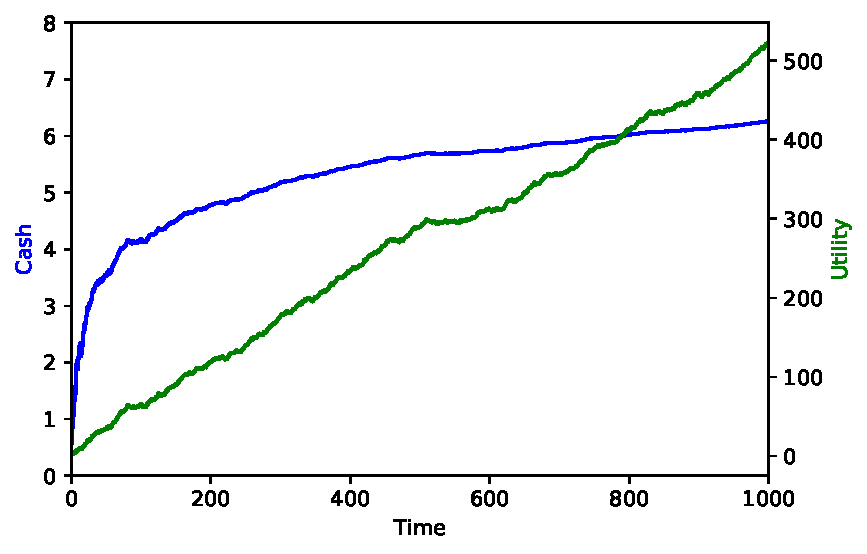
\includegraphics[width=\textwidth]{./chapter_rates/figs/trajectories.pdf}
%}
%\end{picture}
\caption{\small Typical trajectory $\x(\t)$ of the wealth
dynamic \eref{test_dyn}, with parameter values $a_u=1/2$ and $b_u=1$,  and the corresponding Brownian motion $\gu(\t)$. Note that the fluctuations in $\x(\t)$ become smaller for larger wealth. }
\flabel{test_dyn}
\end{figure}

\begin{example}{A curious-looking dynamic}
Given a dynamic, it is possible to check whether it can be mapped into
a utility function, and the utility function itself can be found. We consider the wealth dynamic
\begin{equation}
\gd\x=\left(\frac{a_u}{b_u}e^{-\x}-\frac{1}{2}e^{-2\x}\right)\gd\t+e^{-\x}\gd\gW.
\elabel{test_dyn}
\end{equation}
We note that $a_x(\x)=\frac{a_u}{b_u}e^{-\x}-\frac{1}{2}e^{-2\x}$ and $b_x(\x)=e^{-\x}$.
\Eref{consistency} imposes conditions on the drift term $a_x(\x)$ in terms of the 
noise term $b_x(\x)$. Substituting in \eref{consistency} reveals that the consistency 
condition is satisfied by the dynamic in \eref{test_dyn}.
A typical trajectory of \eref{test_dyn} is shown in \fref{test_dyn}.

Because \eref{test_dyn} is internally consistent, it is possible to derive the corresponding utility function.
\Eref{b_u} is a first-order ordinary differential equation for $\gu(\x)$
\begin{align}
\gu'(\x)=\frac{b_u}{b_x(\x)},
\elabel{diff_eq_u}
\end{align}
which can be integrated to
\begin{align}
\gu(\x)=\int_0^\x \gd\tilde{\x} \frac{b_u}{b_x(\tilde{\x})}+C,
\end{align}
with $C$ an arbitrary constant of integration. This constant, incidentally, implies that 
only {\it changes} in utility are meaningful, as was pointed out by von 
Neumann and Morgenstern \cite{vonNeumannMorgenstern1944} -- this robust feature
is visible whether one thinks in dynamic terms and time averages or in terms of consistent
measure-theoretic concepts and expectation values.

Substituting for $b_x(\x)$ from \eref{test_dyn}, \eref{diff_eq_u} becomes
\begin{equation}
\gu'(\x)=b_u e^\x,
\end{equation}
which is easily integrated to
\begin{equation}
\gu(\x)=b_u e^\x +C,
\elabel{test_dyn_u}
\end{equation}
plotted in \fref{u_of_x}. This exponential utility function is monotonic and therefore invertible -- we knew that because the consistency condition is satisfied. 
The utility function is convex. From the 
perspective of expected-utility theory an individual behaving optimally according to 
this function would be labelled ``risk-seeking.'' 
The dynamical perspective corresponds to a qualitatively different interpretation: 
Under the dynamic \eref{test_dyn} the ``risk-seeking'' individual behaves optimally, 
in the sense that his wealth will grow faster than that of a risk-averse individual. What's optimal is determined by the dynamic, not by the individual. Of course the individual may choose whether to behave optimally. 
The dynamic \eref{test_dyn} has the feature that fluctuations in wealth become smaller
as wealth grows. High wealth is therefore sticky -- an individual will quickly fluctuate out of 
low wealth and into higher wealth. It will then tend to stay there. 
\end{example}

\begin{figure}
\centering
\begin{picture}(200,80)(0,0)
 \put(-80,0){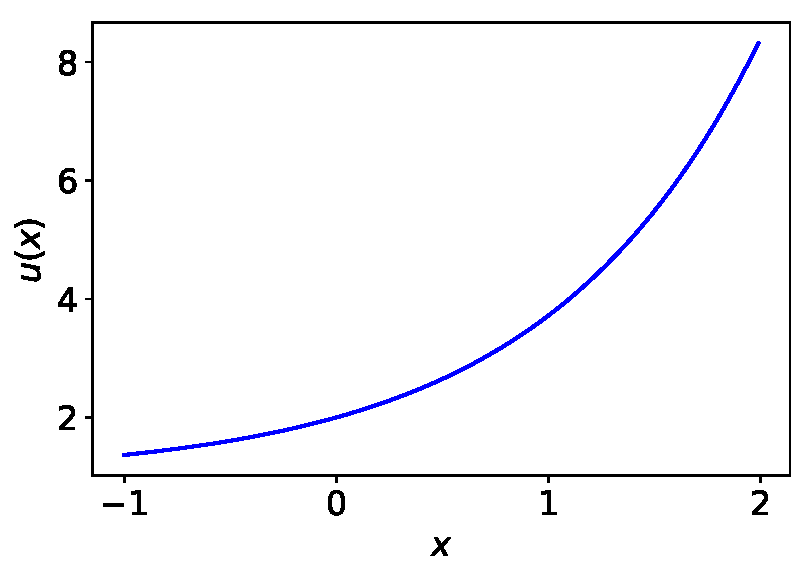
\includegraphics[width=.47\textwidth]{./chapter_rates/figs/u_of_x.pdf}}
 \put(110,0){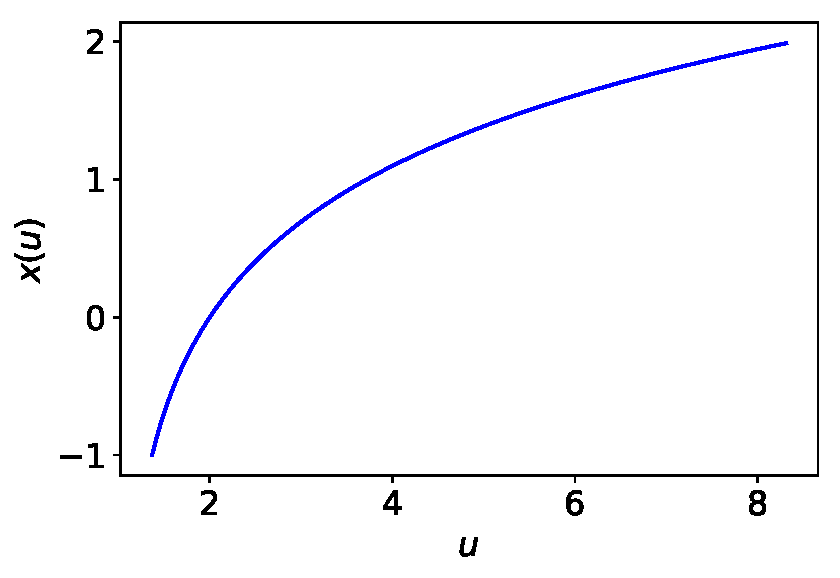
\includegraphics[width=.47\textwidth]{./chapter_rates/figs/x_of_u.pdf}}
\end{picture}
\caption{\small Exponential utility $\gu(\x)$, \eref{test_dyn_u} with $b_u=1$ and $C=1$, is monotonic and unbounded and therefore invertible.
Left panel: $\gu(\x)$. Right panel: inverse $\x(\gu)$.}
\flabel{u_of_x}
\end{figure}
%%%%%%%%%%%%%%%%%%%%%%%%%%%%%%%%%%%%%%%%%%%%%%%
\section{The Copenhagen experiment}
\seclabel{Copenhagen}

XXX TBD XXX

%%%%%%%%%%%%%%%%%%%%%%%%%%%%%%%%%%%%%%%%%%%%%%%
\section{The St Petersburg paradox}
The problem known today as the St Petersburg paradox was suggested by Nicolaus 
Bernoulli\footnote{Daniel's cousin. The Bernoulli family produced a remarkable 
number of famous mathematicians in the $17^\text{th}$ and $18^\text{th}$ centuries, 
who helped lay the foundations of applied mathematics and physics.} in 1713 in his 
correspondence with Montmort~\cite{Montmort1713}. It involves a hypothetical 
lottery for which the rate of change of expected wealth diverges for any finite ticket 
price. The expected-wealth paradigm would predict, therefore, that people are 
prepared to pay any price to enter the lottery. However, when the question is put 
to them, they rarely want to wager more than a few dollars. This 
is the paradox. It is the first well-documented example of the inadequacy of the 
expected-wealth paradigm as a model of human rationality. It was the primary 
motivating example for Daniel Bernoulli's and Cramer's development of the 
expected-utility paradigm~\cite{Bernoulli1738}.

In some sense it is a pity that this deliberately provocative and unrealistic lottery has played such an important role in the development of classical decision theory. It is quite unnecessary to invent a gamble with a diverging change in expected wealth to expose the flaws in the expected-wealth paradigm. The presence of infinities in the problem and its variously proposed solutions has caused much confusion, and permits objections on the grounds of physical impossibility. Such objections are unhelpful because they are not fundamental: they address only the gamble and not the decision paradigm. Nevertheless, the paradox is an indelible part not only of history but also of the current debate~\cite{Peters2011b}, and so we recount it here. We'll start by defining the lottery.

\begin{example}{St Petersburg lottery}
The classical statement of the lottery is to imagine a starting prize 
of $\$1$ (originally the prize was in ducats). A fair coin is tossed: 
if it lands heads, the player wins the prize and the lottery ends; if it lands 
tails, the prize is doubled and the process is repeated. Therefore, the 
player wins $\$2$, $\$4$, $\$8$ if the first head lands 
on the second, third, fourth toss, and so on. The player must buy a ticket, 
at price $\F$, to enter the lottery. The question usually posed is: what is 
the largest $\F$ the player is willing to pay?

The lottery can be translated neatly into our gamble formalism:
\be
\q_\gj = \$ 2^{\gj-1} - \F, \quad \p_\gj = 2^{-\gj},
\elabel{lottery_def}
\ee
for $\gj\in\{1,2,3,\ldots\}$, \ie the set of positive integers. The vast majority 
of observed payouts are small, but occasionally an extremely large payout 
(corresponding to a very long unbroken sequence of tails in the classical 
description) occurs. This is shown in the example trajectories in 
\fref{lottery_add_traj}, where the lottery has been repeated additively.

From now on we will forget about the coin tosses, which are simply a 
mechanism for selecting one of the possible payouts. In effect, they 
are just a random number generator. Instead we shall work with the 
compact definition of the lottery in \eref{lottery_def} and assume it 
takes a fixed amount of time, $\dt$, to play.

The rate of change of expected wealth is
\bea
\frac{\ave{\d\x}}{\dt} & = & \frac{1}{\dt} \sum_{\gj=1}^\infty \p_\gj \q_\gj \\
&=& \frac{1}{\dt} \left( \$ \sum_{\gj=1}^\infty 2^{-\gj}\,2^{\gj-1} - \sum_{\gj=1}^\infty 2^{-\gj} \F \right) \\
&=& \frac{1}{\dt} \left( \$ \sum_{\gj=1}^\infty \frac{1}{2} - \F \right). \elabel{lottery_ex_wealth}
\eea
This diverges for any finite ticket price. Under the expected-wealth paradigm, this means that the lottery is favourable at any price.
\end{example}
\begin{figure}
\centering
\begin{picture}(200,230)(0,0)
\put(-75,0){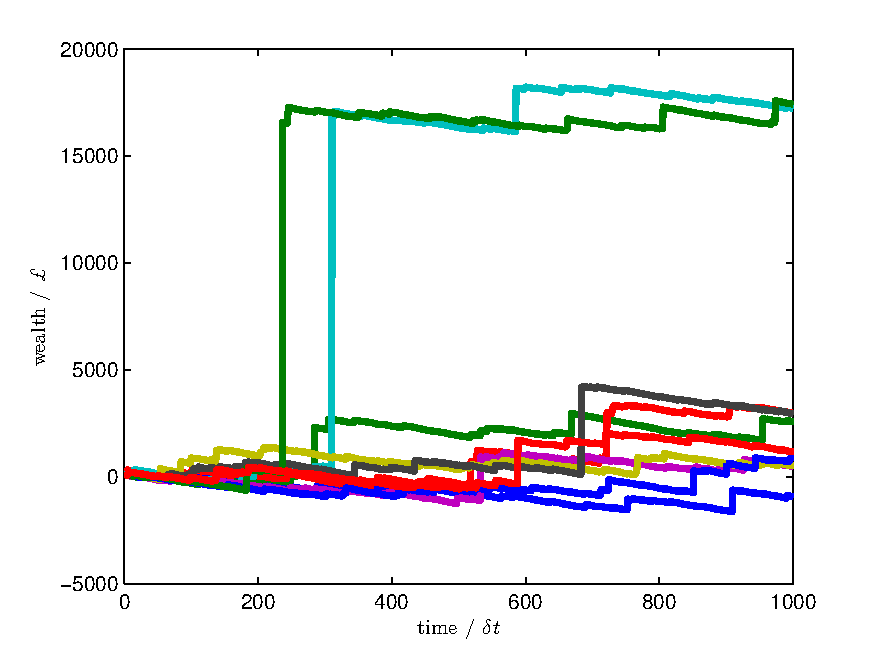
\includegraphics[width=\textwidth]{./chapter_rates/figs/lottery_add_traj.pdf}}
\end{picture}
\caption{Wealth trajectories for the additively repeated St Petersburg lottery, 
with starting wealth, $\x(0)=\$100$, and ticket price, $\F=\$10$. 
Ten trajectories are plotted over 1,000 rounds.\flabel{lottery_add_traj}}
\end{figure}

This implausible conclusion, which does not accord with human behaviour, 
exposes the weakness of judging a gamble by its effect on expected 
wealth. Daniel Bernoulli suggested to resolve the paradox by adopting 
the expected-utility paradigm. His choice of utility function was the 
logarithm, $\gu(\x)=\ln \x$, which, as we now know, produces a decision 
rule equivalent to growth-rate optimisation under multiplicative repetition. 
This correspondence was not appreciated by Bernoulli: indeed $18^\text{th}$-century mathematics did not possesse the concepts and 
language required to distinguish between averages over time and across 
systems, even though it had the basic arithmetic tools. 
%In any case, the 
%correspondence relies on the choice of a particular utility function, and vanishes the moment something other than the logarithm is chosen. We also have
%to interpret expected utility theory a little differently from how it is usually presented -- for instance we have to assume that expected changes in utility really mean expected rates of changes, with a specific gamble duration, \ie we have to introduce the concept of time into utility theory quite differently from that's usually done (which we won't discuss here).

Unfortunately, Bernoulli made a mathematical error in the implementation 
of his own paradigm -- accidentally he proposed two mutually inconsistent versions of utility theory in the paper that established the paradigm. Initially, the error had little impact, and it was corrected by Laplace in 
1814~\cite{Laplace1814}. But Laplace didn't openly say he'd corrected an error, he just worked with what he thought Bernoulli had meant. This politeness had awful consequences. In
1934 Menger~\cite{Menger1934}, keen to get the story right, went back to the original text by Bernoulli. He didn't notice the error but rather got confused by it which led him to introduce a further error. Based on this car crash of scientific communication, Menger derived the infamous (wrong) claim we encountered in \secref{Technical}: utility functions must be bounded, with disastrous consequences for the budding neoclassical formalism. We 
will leave this most chequered part of the paradox's history alone -- details can be found 
in~\cite{PetersGell-Mann2016}. Instead we will focus on what's usually 
presumed Bernoulli meant to write.

\begin{example}{Resolution by logarithmic utility}
Instead of \eref{lottery_ex_wealth}, we calculate the rate of change of expected logarithmic utility,
\bea
\frac{\ave{\d\ln \x}}{\dt} & = & \frac{1}{\dt} \sum_{\gj=1}^\infty \p_\gj \left[\ln(\x+\q_\gj)-\ln \x\right] \\
&=& \frac{1}{\dt} \sum_{\gj=1}^\infty 2^{-\gj} \ln\left(\frac{\x+\$2^{\gj-1}-\F}{\x}\right), \elabel{lottery_ex_util}
\eea
where $\x$ is the ticket buyer's wealth.

This is finite for all finite ticket prices less than the buyer's wealth plus the smallest 
prize: $\F<\x+\$1$. This can be shown by applying the ratio 
test.\footnotemark\ It may be positive or negative, depending on the values 
of $\F$ and $\x$. \fref{gbar_zero} shows the locus of points in the $(\x,\F)$-plane 
for which the sum is zero.
\end{example}
\footnotetext{The ratio of the $(\gj+1)^\text{th}$ term to the $\gj^\text{th}$ term 
in the sum tends to $1/2$ as $\gj\to\infty$.}
\begin{figure}
\centering
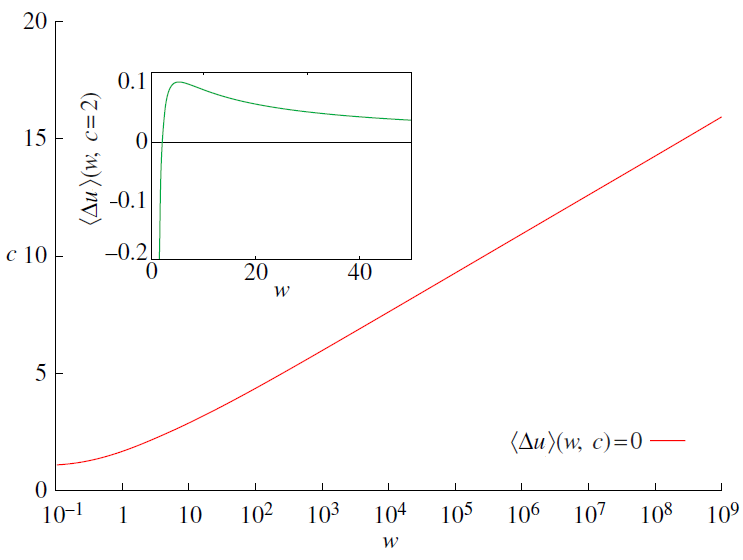
\includegraphics[width=\textwidth]{./chapter_rates/figs/gbar_zero.png}
\caption{Locus of points in the $(\x,\F)$-plane for which the expected change in 
logarithmic utility is zero. The inset shows the expected change in utility as a 
function of $\x$ for $\F=\$2$. Adapted from~\cite{Peters2011b}.\flabel{gbar_zero}}
\end{figure}

The utility paradigm is a model that resolves the paradox, in the sense that creates a world where players may decline to buy a ticket. Bernoulli argued for this resolution framework in plausible terms: the usefulness of a monetary gain depends on how much money you already have. He also argued specifically for the logarithm in plausible terms: the gain in usefulness should be proportional to the fractional gain it represents, $\d \gu = \d\x/\x$. Yet, the framework has left many unsatisfied: why does usefulness have this functional form? We provide this deeper reason by connecting the problem to dynamics and time, unlike Bernoulli. Had Bernoulli made the connection, he might have been less willing to accept Cramer's square-root utility function as an alternative, which, as we've seen, corresponds to a rather less intuitive dynamic.

%However, while plausible, the framework relies on a utility function, which must be postulated. It can neither be derived from fundamental considerations nor verified empirically.

Turning to our decision algorithm, we will assume that the lottery is repeated multiplicatively. This means, in effect, that the prizes and ticket price are treated as fractions of the player's wealth, such that the effect of each lottery is to multiply current wealth by a random factor,
\be
\gr_\gj = \frac{\x+\$2^{\gj-1}-\F}{\x}, \quad \p_\gj= 2^{-\gj}.
\ee
This follows precisely our earlier treatment of a gamble with multiplicative dynamics, and we can apply our results directly. 
The time-average (exponential) growth rate is
\be
\gt_\text{m} = \frac{1}{\dt} \lim_{\T\to\infty} \left\{ \frac{1}{\T}  \sum_{\gtau=1}^\T \ln \gr(\gtau) \right\} = \frac{1}{\dt}  \sum_{\gj=1}^\infty 2^{-\gj} \ln \gr_\gj, \elabel{lottery_gbar}
\ee
which is identical to the expression for the rate of change of expected log-utility, 
\eref{lottery_ex_util}. This is, as we've discussed, because $\gv(\x)=\ln(\x)$ 
is the appropriate ergodicity mapping for multiplicative dynamics. The result is the same, but 
the interpretation is different: we have assumed less, only that our player is 
interested in the growth rate of his wealth and that he gauges this by imagining 
the outcome of an indefinite sequence of repeated lotteries.

Thus the locus in \fref{gbar_zero} also marks the decision threshold \textit{versus} 
the null gamble under our decision axiom. The player can sensibly decline the 
gamble, even though it results in a divergent change in expected wealth. This 
is illustrated by comparing \fref{lottery_mult_traj}, which shows trajectories of 
multiplicatively repeated lotteries, with the additively repeated lotteries already 
seen in \fref{lottery_add_traj}.
\begin{figure}
\centering
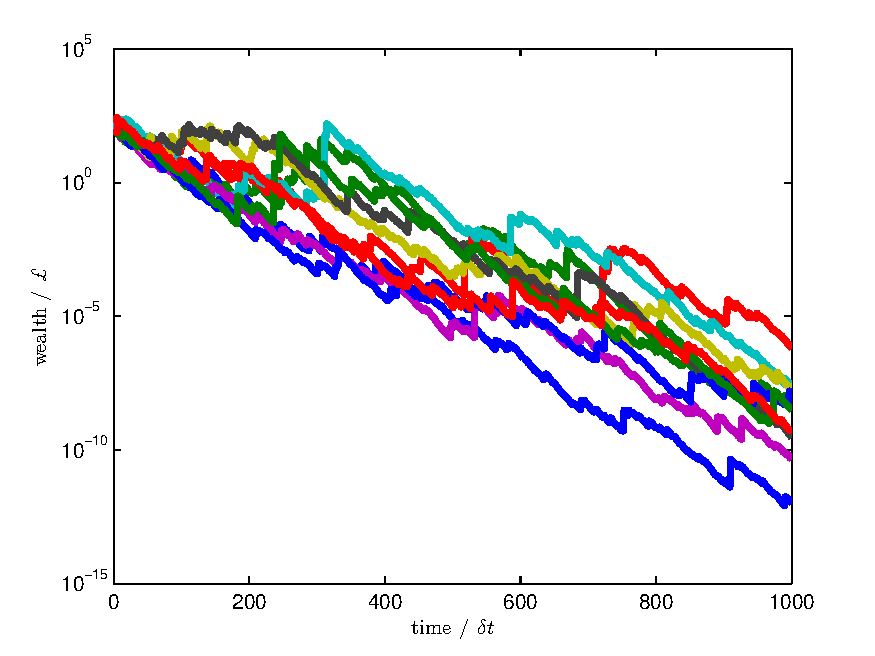
\includegraphics[width=\textwidth]{./chapter_rates/figs/lottery_mult_traj.pdf}
\caption{Wealth trajectories for the multiplicatively repeated St Petersburg lottery, 
with starting wealth, $\x(0)=\$100$, and ticket price, $\F=\$10$. Ten 
trajectories are plotted over 1,000 rounds. The realisations of the individual 
lotteries are the same as in \fref{lottery_add_traj} but the mode of repetition is 
different.\flabel{lottery_mult_traj}}
\end{figure}
The trajectories are based on the same sequences of lottery outcomes, only 
the mode of repetition is different. The simulation shows us visually what we 
have already gleaned by analysis: what appears favourable in the 
expected-wealth paradigm (corresponding to additive repetition) results in a 
disastrous decay of the player's wealth over time under a realistic dynamic.

As $\F\to \x+\$1$ from above in \eref{lottery_gbar}, $\gt_\text{m}$ diverges 
negatively, since the first term in the sum is the logarithm of a quantity approaching 
zero. This corresponds to a lottery which can make the player bankrupt. The effect 
is also shown in the inset of \fref{gbar_zero}.

Treatments based on multiplicative repetition have appeared sporadically in the 
literature, starting with Whitworth in 
1870~\cite[App.~IV]{Whitworth1870}.\footnote{Whitworth was dismissive of early utility theory: ``The result at which we have arrived is not to be classed with 
the arbitrary methods which have been again and again propounded to evade the difficulty of the Petersburg problem\ldots. Formulae have often been proposed, which have possessed the one virtue of presenting a finite result\ldots but they have often had no intelligible basis to rest upon, or\ldots sufficient care has not been taken to draw a distinguishing line between the significance of the result obtained, and the different result arrived at when the mathematical expectation is calculated.'' Sadly he chose to place these revolutionary remarks in an appendix of a college probability textbook.} It is related to the famous Kelly Criterion~\cite{Kelly1956}\footnote{Kelly was similarly unimpressed with the mainstream and noted in his treatment of decision theory, which he developed from the perspective of information theory and which is identical to ergodicity economics with multiplicative dynamics, that the utility function is ``too general to shed any light on the specific problems of communication theory.''}, although Kelly did not explicitly treat the St Petersburg game, and tangentially to \Ito's lemma~\cite{Ito1944}. It appears as an exercise in a well-known text on information theory~\cite[Ex.~6.17]{CoverThomas1991}. Mainstream economics has ignored all this. A full and rigorous resolution of the paradox, including the epistemological significance of the shift from ensemble to time averages, was published recently by one of the present authors~\cite{Peters2011b}.

%%%%%%%%%%%%%%%%%%%%%%%%%%%%%%%%%%%%%%%%%%%%%%%
\section{The insurance puzzle}
The insurance contract is an important and ubiquitous type of economic transaction, 
which can be modelled as a gamble. However, it poses a 
puzzle~\cite{PetersAdamou2015b}. In the expected-wealth paradigm, insurance 
contracts shouldn't exist, because buying insurance would only be rational at a 
price at which it would be irrational to sell. More specifically:
\begin{enumerate}
\item To be viable, an insurer must charge an insurance premium of at least the 
expectation value of any claims that may be made against it, called the ``net 
premium'' \cite[p.~1]{KaasETAL2008}.
\item The insurance buyer therefore has to be willing to pay more than the net 
premium so that an insurance contract may be successfully signed.
\item Under the expected-wealth paradigm it is irrational to pay more than the 
net premium, and therefore insurance contracts should not exist.
\end{enumerate}
In this picture, an insurance contract can only ever be beneficial to one party. It 
has the anti-symmetric property that the expectation value of one party's gain is 
the expectation value of the other party's loss.

The puzzle is that insurance contracts are observed to exist.\footnote{Something 
of an understatement. The Bank for International Settlements estimated the 
market value of all the world's derivatives contracts, which are essentially 
insurance contracts, as \$15 trillion in the first half of 2015 (see 
\url{http://www.bis.org/statistics/d5\_1.pdf}). That's six times the gross domestic 
product of the United Kingdom.} Why? Classical resolutions appeal to utility 
theory (\ie psychology) and asymmetric information (\ie deception). However, 
our decision theory naturally predicts contracts with a range of prices that 
increase the time-average growth rate for both buyer and seller. We illustrate 
this with an example drawn from maritime trade, in which the use of insurance 
has a very long history.\footnote{Contracts between Babylonian traders and 
lenders were recorded around 1750 BC in the Code of Hammurabi. Chinese 
traders practised diversification by spreading cargoes across multiple vessels 
even earlier than this, in the third millennium BC.} A similar 
example was used by Bernoulli~\cite{Bernoulli1738}.

\begin{example}{A shipping contract}
We imagine a shipowner sending a cargo from St Petersburg to Amsterdam, with the following parameters:
\begin{itemize}
\item owner's wealth, $\x_\text{own}=\$100,000$;
\item gain on safe arrival of cargo, $\G=\$4,000$;
\item probability ship will be lost, $\p=0.05$;
\item replacement cost of the ship, $\C=\$30,000$; and
\item voyage time, $\dt=1$ month.
\end{itemize}
An insurer with wealth $\x_\text{ins}=\$1,000,000$ proposes to insure the voyage for a 
fee, $\F=\$1,800$. If the ship is lost, the insurer pays the owner $\gL=\G+\C$ to make him 
good on the loss of his ship and the profit he would have made.
\end{example}
We phrase the decision the owner is facing as a choice between 
two gambles. 

\begin{definition}{The owner's gambles}

Sending the ship uninsured corresponds to gamble o1
\bea
\q_1^{(\text{o1})} = \G, &\quad& \p_1^{(\text{o1})} = 1-p;\\
\q_2^{(\text{o1})} = -\C, &\quad& \p_2^{(\text{o1})} = p.
\eea
Sending the ship fully insured corresponds to gamble o2
\bea
\q_1^{(\text{o2})} = \G-\F &\quad& \p_1^{(\text{o2})} = 1.
\eea
This is a trivial ``gamble'' because all risk has been 
transferred to the insurer. 
\end{definition}

We also model the insurer's decision whether to offer the contract as
a choice between two gambles

\begin{definition}{The insurer's gambles}

Not insuring the ship corresponds to gamble i1, which is the null gamble
\bea
\q_1^{(\text{i1})} = 0 &\quad& \p_1^{(\text{i1})} = 1.
\eea

Insuring the ship corresponds to gamble i2
\bea
\q_1^{(\text{i2})} = +\F, &\quad& \p_1^{(\text{i2})} = 1-p;\\
\q_2^{(\text{i2})} = -\gL+\F, &\quad& \p_2^{(\text{i2})} = p.
\eea
\end{definition}

We ask whether the owner should sign the contract, and whether the insurer should have proposed it.

\begin{example}{Expected-wealth paradigm}
In the expected-wealth paradigm (corresponding to additive repetition under 
the time paradigm) decision makers
maximise the rate of change of the expectation values of their wealths, according to \eref{ex_crit}:
Under this paradigm the owner collapses gamble o1 into the scalar

\bea
\gt_a^{(\text{o1})} &=& \frac{\ave{\d\x}}{\dt}\\
&=&\frac{\ave{\q^{(\text{o1})}}}{\dt}\\
&=&\frac{(1-p) \G + p (-\C) }{\dt}\\
&=&\$ 2,300\text{ per month,}
\eea

and gamble o2 into the scalar

\bea
\gt_a^{\text{o2}} &=&\frac{\ave{\q^{(\text{o2})}}}{\dt}\\
&=&\frac{(\G-\F) }{\dt}\\
&=&\$2,200 \text{ per month.}
\eea
The difference, $\delta\gt_a^\text{o}$,  between the expected rates 
of change in wealth with and without a signed contract is the expected 
loss minus the fee per round trip,
\be
\delta\gt_a^\text{o}=\gt_a^{\text{o2}}-\gt_a^{\text{o1}}= \frac{\p \gL - \F}{\dt}.
\elabel{dro}
\ee
The sign of this difference indicates whether the insurance contract is beneficial
to the owner. In the example this is not the case, $\delta\gt_a^\text{o}=-\$100$ per month.

The insurer evaluates the gambles i1 and i2 similarly, with the result
\be
\gt_a^{(\text{i1})}  = \$0 \text{ per month,}
\ee
and
\bea
\gt_a^{(\text{i2})}  &=& \frac{\F-\p \gL}{\dt} \elabel{r}\\ 
&=& \$100 \text{ per month.}
\eea
Again we compute the difference -- the net benefit to the insurer that arises from signing the contract
\be
\delta\gt_a^\text{i}=\gt_a^{\text{i2}}-\gt_a^{\text{i1}}= \frac{\F- \p \gL}{\dt}.
\elabel{dri}
\ee
In the example this is $\delta\gt_a^\text{i}=\$100$ per month, meaning that in the 
world of the expected-wealth paradigm the insurer will offer the contract.
\end{example}

Because only one party (the insurer) is willing to sign, no contract will come into existence. We could think that we got
the price wrong, and the contract would be sigend if offered at a different fee. 
But this is not the case, and that's the fundamental insurance puzzle: in the
world created by expected-wealth maximisation no price exists at which both
parties will sign the contract.

Looking at \eref{dro} and \eref{dri} we notice the anti-symmetric relationship between
the two expressions,  
$\delta\gt_a^\text{o}=-\delta\gt_a^\text{i}$.
By symmetry, there can be no fee at which both expressions are positive. 
Hence there are no circumstances in the world created by the 
expected-wealth paradigm under which both parties will sign. Insurance
contracts cannot exist in this world.

One party winning at the expense of the other makes insurance an 
unsavoury business in the expected-wealth paradigm. This is further 
illustrated in \fref{ins_lin}, which shows the change in the rate of 
change of expected wealth (the decision variable) for both parties 
as a function of the fee, $\F$.
\begin{figure}
\centering
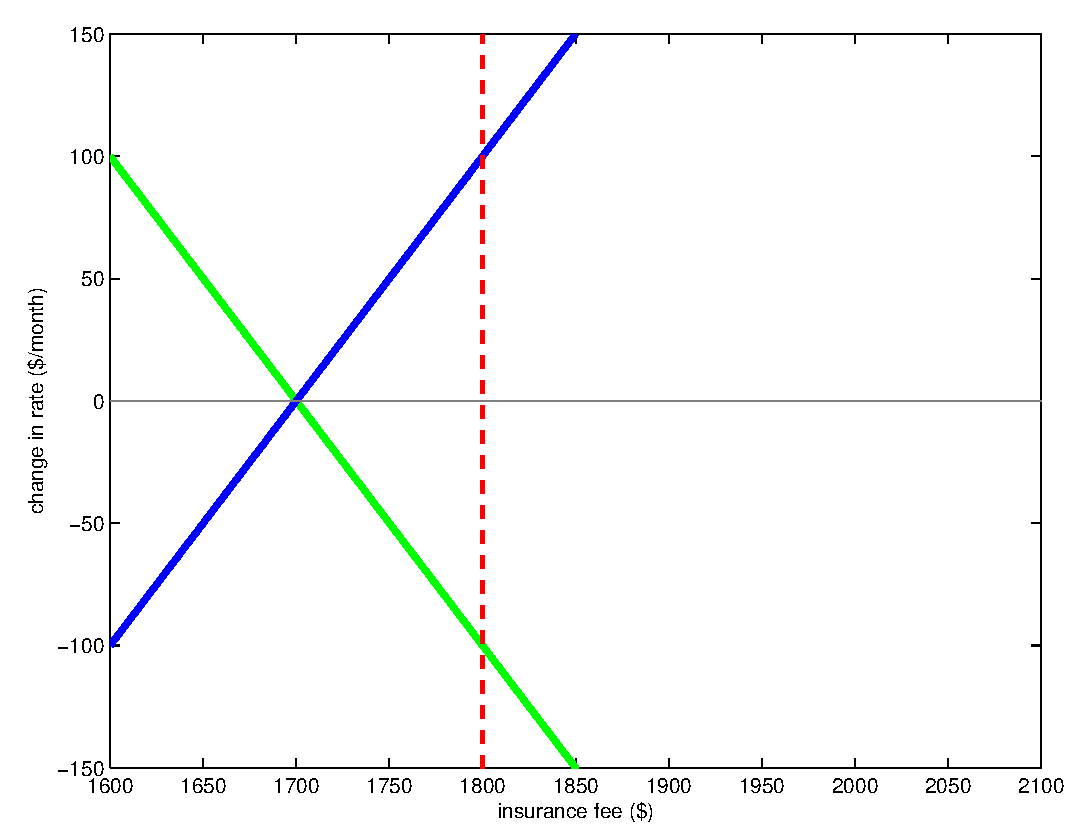
\includegraphics[width=\textwidth]{./chapter_rates/figs/ins_lin_cropped.pdf}
\caption{Change in the rate of change of expected wealth for the shipowner (green) and the 
insurer (blue) as a function of the insurance fee, $\F$.\flabel{ins_lin}}
\end{figure}
There is no price at which the decision variable is positive for the both parties. The best they can 
do is to pick the price at which neither of them cares whether they sign or not.

In this picture, the existence of insurance contracts requires some asymmetry between the contracting parties, such as:
\begin{itemize}
\item different attitudes to bearing risk;
\item different access to information about the voyage;
\item different assessments of the riskiness of the voyage;
\item one party to deceive, coerce, or gull the other into a bad decision.
\end{itemize}
It is difficult to believe that this is truly the basis for a market of the size and global reach of the insurance market.

\subsection{Solution in the time paradigm}

\begin{example}{Time paradigm}
The insurance puzzle is resolved in the `time paradigm', \ie using 
the growth-optimal decision theory we have developed in this lecture
and multiplicative repetition. Again, we pause to reflect what multiplicative
repetition means compared to additive repetition. This is important because
additive repetition is equivalent to the expected-wealth paradigm that 
created the insurance puzzle.  Multiplicative repetition means that the 
ship owner sends out a ship and a cargo whose values are proportional to 
his wealth at the start of each voyage. A rich owner who has had many 
successful voyages will send out more cargo, a larger ship, or perhaps a \textit{flotilla}, while an owner 
to whom the sea has been a cruel mistress will send out a small vessel until his luck changes.
Under additive repetition, the ship owner would send out the same amount
of cargo on each journey, irrespective of his wealth. Shipping companies
of the size of Evergreen or Maersk would be inconceivable under additive repetition,
where returns on successful investments are not reinvested.

The two parties seek to maximise
\be
\gt_m = \lim_{\Dt\to\infty}\frac{\D\gv(\x)}{\Dt} = \frac{\ave{\d\ln \x}}{\dt},
\ee
where we have used the ergodic property of $\D\gv(\x)=\D\ln\x$
under multiplicative repetition.

The owner's time-average growth rate without insurance is 
\be
\gt_m^\text{o1} = \frac{(1-\p)\ln(\x_\text{own}+\G)+\p\ln(\x_\text{own}-\C) - \ln(\x_\text{own})}{\dt}
\ee
or 1.9\% per month. 
His time-average growth rate with insurance is 
\be
\gt_m^\text{o2} = \frac{\ln(\x_\text{own}+\G-\F)-\ln(\x_\text{own})}{\dt}
\ee
or 2.2\% per month. This gives a net benefit for the owner of
\be
\d\gt_m^o = \gt_m^\text{o1}-\gt_m^\text{o2} \approx +0.24\% \text{ per month.} 
\ee
The time paradigm thus creates a world where the owner will sign the contract.

What about the insurer? Without insurance, the insurer plays the null gamble, and
\be
\gt_m^{\text{i1}}= \frac{0}{\dt}
\ee
or 0\% per month. His time-average growth rate with insurance is 
\be
\gt_m^{\text{i2}} = \frac{(1-p)\ln(\x_\text{ins}+\F) + p\ln(\x_\text{ins}+\F-\gL) - \ln(\x_\text{ins})}{\dt}
\ee
or 0.0071\% per month. The net benefit to the insurer is therefore also
\be
\delta\gbar_m^{\text{i}} = \gt_m^{\text{i2}}-\gt_m^{\text{i1}}
\ee
\ie 0.0071\% per month. Unlike the expected wealth paradigm, the time paradigm with multiplicative repetition 
creates a world where an insurance contract can exist -- there exists a range of fees $\F$ at which
both parties gain from signing the contract! 
\end{example}


We view this as the
\begin{keypts}{Fundamental resolution of the insurance puzzle:}
The buyer and seller of an insurance contract both sign when it increases the time-average growth rates of their wealths.
\end{keypts}
It requires no appeal to arbitrary utility functions or asymmetric circumstances, rather it arises naturally from the model of human decision-making that we have set out. \fref{ins_log} shows the mutually beneficial range of insurance fees predicted by our model.
\begin{figure}
\centering
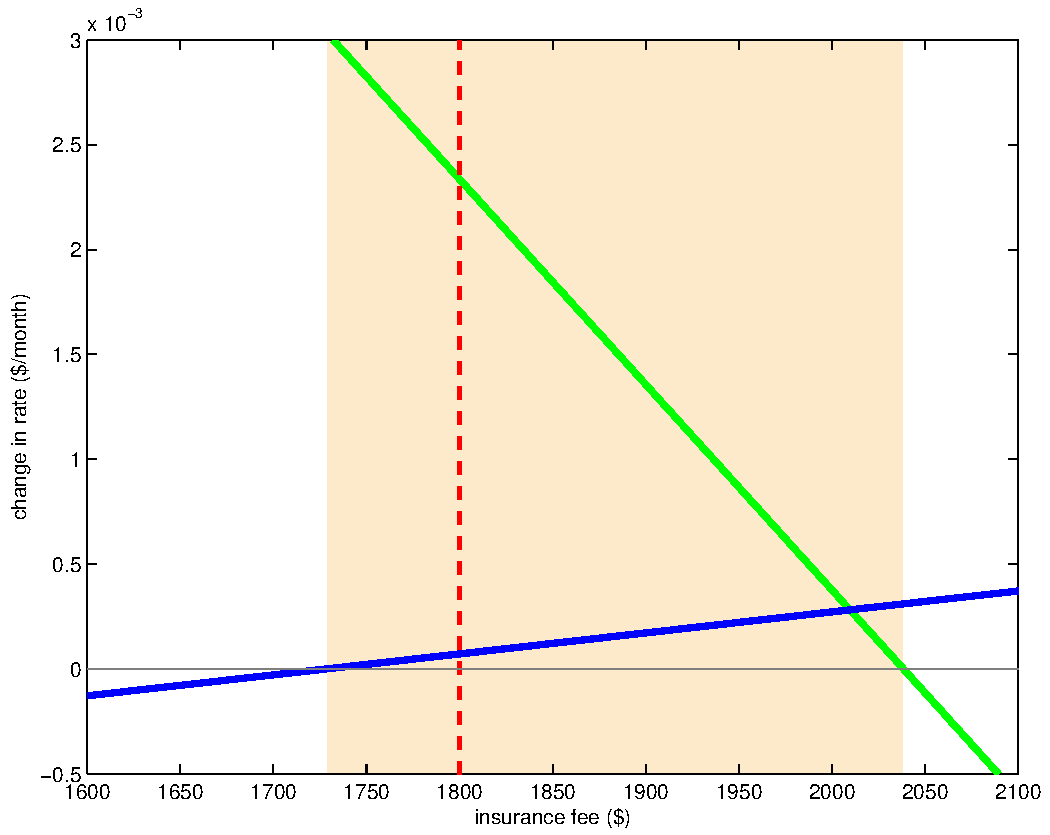
\includegraphics[width=\textwidth]{./chapter_rates/figs/ins_log_cropped.pdf}
\caption{Change in the time-average growth rate of wealth for the shipowner (green) and the insurer (blue) as a function of the insurance fee, $F$. The mutually beneficial fee range is marked by the beige background.\flabel{ins_log}}
\end{figure}
Generalizing, the message of the time paradigm is that business happens when both parties gain.
In the world created by this model any agreement, any contract, any commercial interaction 
comes into existence because it is mutually beneficial.

%\printglossary[title=Glossary,type=\acronymtype]
%%
%\printglossary[title=List of Symbols]
\subsection{The classical solution of the insurance puzzle}
\seclabel{The classical solution of the insurance puzzle}

%\begin{example}{Expected-utility paradigm}
%Let's look at the solution in the expected-utility paradigm. Our players now seek to maximise the rate of change of their expected utility,
%\be
%\ave{r_u} \equiv \frac{\ave{\Du(W)}}{\Dt}.
%\ee
%To make the example concrete, we will use $u(W)=\sqrt{W}$, as suggested by Cramer~\cite{Cramer1728}, for both parties.
%
%The owner has
%\be
%\ave{r_u}_\text{own}^\text{un} = \frac{(1-p)u(W_\text{own}+G)+pu(W_\text{own}-C) - u(W_\text{own})}{\Dt}
%\ee
%or 3.37 `utils'\footnotemark\ per month without insurance, and 
%\be
%\ave{r_u}_\text{own}^\text{in} = \frac{u(W_\text{own}+G-F)-u(W_\text{own})}{\Dt}
%\ee
%or 3.46 utils per month with insurance. The change in $\ave{r_u}_\text{own}$ is 
%\be
%\delta\ave{r_u}_\text{own} = \ave{r_u}_\text{own}^\text{in} - \ave{r_u}_\text{own}^\text{un},
%\ee
%\ie 0.094 utils per month, and the owner should sign.
%
%The contract is also favourable from the insurer's perspective. If he does no business, then 
%\be
%\ave{r_u}_\text{ins}^\text{un} = \frac{0}{\Dt}
%\ee
%or zero utils per month. If he extends insurance, then
%\be
%\ave{r_u}_\text{ins}^\text{in} = \frac{(1-p)u(W_\text{ins}+F) + pu(W_\text{ins}+F-L) - u(W_\text{ins})}{\Dt}
%\ee
%or 0.043 utils per month and his change in $\ave{r_u}_\text{ins}$ is positive:
%\be
%\quad \delta\ave{r_u}_\text{ins} = \ave{r_u}_\text{ins}^\text{in} - \ave{r_u}_\text{ins}^\text{un},
%\ee
%\ie 0.043 utils per month.
%\end{example}
%\footnotetext{The general unit of utility. Here $1\,\text{util} = \sqrt{\$}\,1$, whatever that might mean.}
The classical solution of the insurance puzzle is identical to the classical solution of the St Petersburg paradox.
Wealth is replaced by a non-linear utility function of wealth, which breaks the symmetry of the 
expected-wealth paradigm. While it is always true that $\delta\ave{r}_\text{own}=-\delta\ave{r}_\text{ins}$, 
the expected growth rates of non-linear utility functions don't share this anti-symmetry. A difference in 
the decision makers' wealths is sufficient, though often different utility functions are assumed for owner and insurer, 
which is a model that can create pretty much any behavior. The downside of a model with this ability is, of course, 
that it makes no predictions -- nothing is ruled out, so the model cannot be falsified.
%
%This represents the classical resolution of the insurance puzzle. The symmetry broken by the different wealths $W_\text{own}$ and $W_\text{ins}$, which now appear in $\ave{r_u}$ since the utility function is nonlinear.\footnote{Note that the symmetry could also have been broken by assigning different utility functions to the two parties, even if their wealths were the same. However, it suffices only that their wealths be different for the puzzle to be resolved.} Certain combinations of $W_\text{own}$, $W_\text{ins}$, and $u$ will admit a range of mutually beneficial prices, $F$. This is visible as the beige region in \fref{ins_sqrt}, which plots the decision variable, $\delta\ave{r_u}$, for both parties as a function of the fee, $F$.
%\begin{figure}
%\centering
%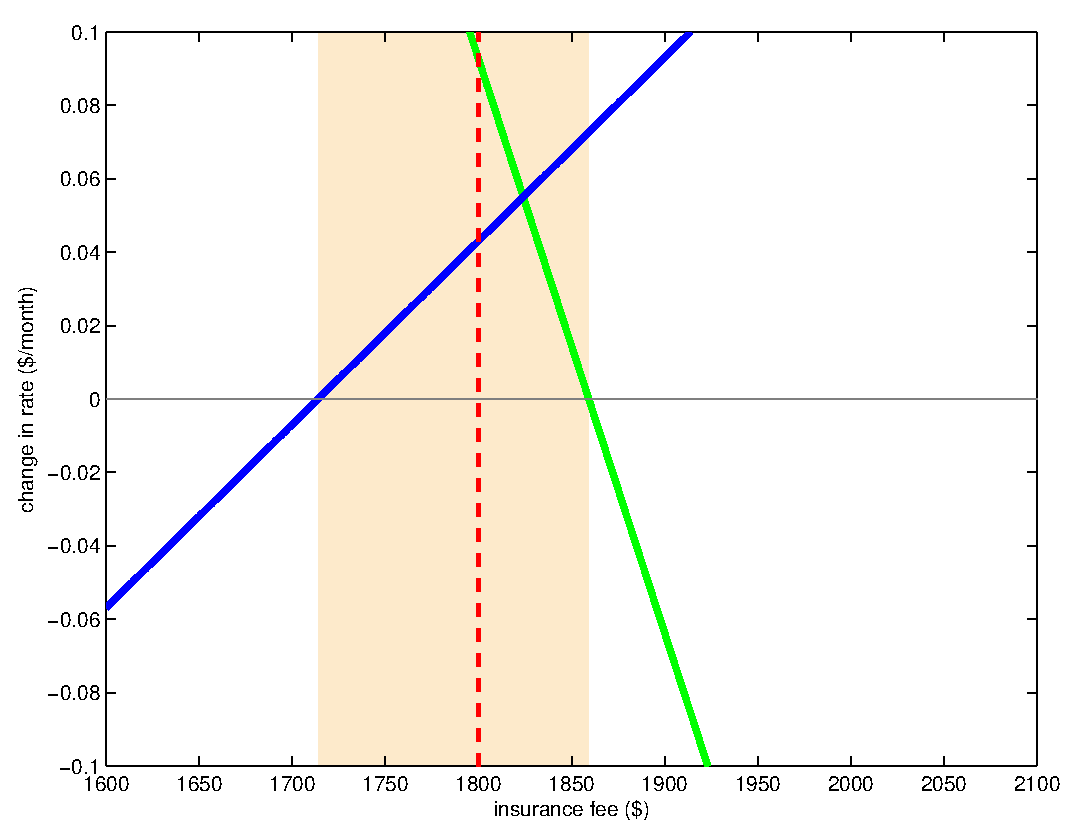
\includegraphics[width=\textwidth]{./chapter_rates/figs/ins_sqrt_cropped.pdf}
%\caption{Change in the rate of change of expected square-root utility for the shipowner (green) and the insurer (blue) as a function of the insurance fee, $F$. The mutually beneficial fee range is marked by the beige background.\flabel{ins_sqrt}}
%\end{figure}
%Utility theory does not rule out insurance contracts -- it is {\it possible} to create a win-win deal -- but does not rule them in either. Furthermore, invoking arbitrary and unobservable utility functions hardly seems a satisfying resolution of the puzzle.